
\documentclass[11pt,oneside]{article}
\usepackage[T1]{fontenc}
\usepackage[utf8]{inputenc}
\usepackage{lmodern}
\usepackage[margin=0.88in]{geometry}
\usepackage{microtype}
\usepackage{amsmath,amssymb,amsthm,mathtools}
\usepackage{booktabs,longtable,tabularx,array}
\usepackage{enumitem}
\usepackage{xcolor}
\usepackage{listings}
\usepackage{fancyhdr}
\usepackage{hyperref}
\usepackage[nameinlink,noabbrev]{cleveref}
\usepackage{tikz}
\usetikzlibrary{arrows.meta,positioning,shapes.geometric,fit,calc}
\usepackage{caption}
\usepackage{url}

\definecolor{linkblue}{RGB}{28,78,135}
\definecolor{deepgreen}{RGB}{25,99,79}
\definecolor{warmred}{RGB}{153,57,44}
\definecolor{codegray}{RGB}{247,247,247}
\definecolor{softblue}{RGB}{238,245,252}
\definecolor{softgreen}{RGB}{239,248,244}
\hypersetup{
  colorlinks=true,
  linkcolor=linkblue,
  citecolor=linkblue,
  urlcolor=linkblue,
  pdftitle={Proof-Carrying Finitary Modules for iPRA},
  pdfauthor={OpenAI research synthesis for Vladimir Reshetnikov and ProveIt}
}
\setlength{\parindent}{0pt}
\setlength{\parskip}{0.52em}
\setlength{\headheight}{14pt}
\setlength{\emergencystretch}{3em}
\setcounter{tocdepth}{2}
\setcounter{secnumdepth}{3}
\setlist[itemize,enumerate]{leftmargin=*,topsep=0.25em,itemsep=0.16em}
\pagestyle{fancy}
\fancyhf{}
\fancyhead[L]{Proof-Carrying Finitary Modules for iPRA}
\fancyhead[R]{\thepage}
\renewcommand{\headrulewidth}{0.4pt}

\lstset{
  basicstyle=\ttfamily\small,
  backgroundcolor=\color{codegray},
  frame=single,
  breaklines=true,
  columns=fullflexible,
  keepspaces=true,
  showstringspaces=false,
  keywordstyle=\bfseries\color{linkblue},
  commentstyle=\itshape\color{deepgreen},
  numbers=left,
  numberstyle=\tiny,
  xleftmargin=1.4em,
  framexleftmargin=1.1em
}

\newtheorem{theorem}{Theorem}[section]
\newtheorem{lemma}[theorem]{Lemma}
\newtheorem{proposition}[theorem]{Proposition}
\newtheorem{corollary}[theorem]{Corollary}
\newtheorem{definition}[theorem]{Definition}
\newtheorem{principle}[theorem]{Principle}
\newtheorem{barrier}[theorem]{Barrier}
\newtheorem{example}[theorem]{Example}
\theoremstyle{remark}
\newtheorem{remark}[theorem]{Remark}
\newtheorem{status}[theorem]{Status}
\newtheorem{roadmap}[theorem]{Lean roadmap}

\newcommand{\iPRA}{\mathrm{iPRA}}
\newcommand{\PRA}{\mathrm{PRA}}
\newcommand{\Nat}{\mathbb{N}}
\newcommand{\Z}{\mathbb{Z}}
\newcommand{\Q}{\mathbb{Q}}
\newcommand{\Bool}{\mathbb{B}}
\newcommand{\PCFM}{\mathsf{PCFM}}
\newcommand{\Prf}{\mathsf{Prf}}
\newcommand{\PRAAx}{\mathsf{PRAAx}}
\newcommand{\PTm}{\mathsf{PTm}}
\newcommand{\Fm}{\mathsf{Fm}}
\newcommand{\Valid}{\mathsf{Valid}}
\newcommand{\ValidObs}{\mathsf{ValidObs}}
\newcommand{\Eqv}{\mathsf{Eqv}}
\newcommand{\Obs}{\mathsf{Obs}}
\newcommand{\CertCheck}{\mathsf{Check}}
\newcommand{\Run}{\mathsf{Run}}
\newcommand{\Inv}{\mathsf{Inv}}
\newcommand{\Post}{\mathsf{Post}}
\newcommand{\Need}{\mathsf{Need}}
\newcommand{\Viable}{\mathsf{Viable}}
\newcommand{\Good}{\mathsf{Good}}
\newcommand{\Guard}{\mathsf{Guard}}
\newcommand{\Res}{\mathsf{Res}}
\newcommand{\code}[1]{\texttt{\detokenize{#1}}}
\newcommand{\defeq}{\mathrel{:=}}
\newcommand{\imp}{\rightarrow}
\newcommand{\iffc}{\leftrightarrow}
\newcommand{\dotminus}{\mathbin{\dot{-}}}

\title{\textbf{Proof-Carrying Finitary Modules}\\[0.22em]
A Shallow Object-Theory Framework for Embedding Mathematics\\
in Intuitionistic Primitive Recursive Arithmetic}
\author{Research synthesis prepared for Vladimir Reshetnikov\\
and the ProveIt iPRA development}
\date{16 November 2026\\
Repository baseline: \texttt{7fa3ba48e8f62e8018ed954faaa48b908217eaf1}}

\begin{document}
\maketitle

\begin{abstract}
The ProveIt iPRA directory contains a mature checked logical kernel and arithmetic library, together with a much larger collection of theorem packets and general frameworks whose mathematical content is mostly not yet connected to kernel-checked object-theory derivations.  This report develops \emph{Proof-Carrying Finitary Modules} (PCFM), a deliberately shallow framework designed to close that gap.

A PCFM module is not merely a program, a semantic contract, or a host-language proposition.  It contains a literal derivation of type
\[
   \Delta,\Gamma\ \vdash_{\PRAAx}\ \varphi
\]
in the ordinary \code{Prf PRAAx} calculus.  Here $\Gamma$ is the local input contract and $\Delta$ is an explicit list of residual producer obligations such as a convergence modulus, a height cutoff, a separation gap, a finite-cover margin, or a correctness theorem for an external certificate.  Modules specialize by \code{Prf.subst}, compose by \code{Prf.trans}, and remain conditional until every residual obligation has itself been supplied by a proof-carrying module.

The main conceptual change is that PCFM is a \emph{shallow typed embedding}.  A fixed theorem-specific proof graph is assembled by Lean functions whose result type is already a \code{Prf PRAAx} judgment.  There is no object-level universal evaluator and no need to prove soundness of a large deep intermediate language before any application can be checked.  Fixed bounded loops are compiled to primitive recursion with one quantifier-free invariant; branches use a recursive Boolean reflection theorem for quantifier-free formulas; bounded existential claims use the checked least-search backend; finite relational choices use backward viability; and exact, quotient-stable, or error-stable observations erase irrelevant witness choices.  A finite-use compilation theorem shows that every well-typed finite graph built from these modules yields a derivation whose hypotheses are exactly its unresolved producer boundaries.

We give complete human-readable proofs of the structural module calculus, quantifier-free Boolean reflection, bounded quantifier elimination, fixed trace reflection, finite relational viability, stable witness erasure, resource-demand composition, and the reduction of open-sequent bridge transport to the existing free-environment translations plus a single code-normalization theorem.  We then instantiate the framework for exact algebra, rational analysis, Cauchy names, finite topology, algebraic geometry by certified setoids, bounded Diophantine search, finite probability approximations, and special-function identities.  The framework resolves several recurring formalization difficulties, while sharply preserving the genuine barriers: a cardinality bound does not give a search cutoff; pointwise convergence does not give a primitive-recursive modulus; a finite compatible family need not yield a coherent infinite selector; exact branch choice fails at collisions without a gap; and unrestricted height bounds for general Faltings- or Siegel-type statements are not manufactured by compilation.

The archive includes the article source and PDF, Lean-oriented module skeletons with exact proposed theorem signatures, an implementation dependency ledger, and executable exact-arithmetic regression tests.  The current artifact does not claim that its Lean skeletons have been compiled; it specifies a path in which each completed file becomes independently kernel-checkable against the current \code{ConciseIPRA}, \code{IPRADerivations}, and \code{IPRABridge} APIs.
\end{abstract}

\begin{center}
\fcolorbox{linkblue}{softblue}{\parbox{0.92\textwidth}{
\textbf{Central deliverable.}
The first implementation target is not another universal proof language.  It is a small library of typed constructors that return actual \(\Prf\,\PRAAx\) terms: structural composition, Boolean reflection, trace induction, bounded search, viability, stable observation, and residual discharge.  Each theorem packet can then migrate one proof boundary at a time.
}}
\end{center}

\tableofcontents
\newpage


\section{Repository baseline and the actual gap}
\label{sec:audit}

\subsection{Four layers that must not be conflated}

At the pinned repository baseline, the iPRA work has four logically different
layers.

\begin{enumerate}
\item
\textbf{The object theory.}
\code{ConciseIPRA} defines the ordinary first-order presentation of iPRA:
primitive-recursive function symbols \code{PR}, terms \code{PTm}, formulas
\code{Fm}, the axiom family \code{PRAAx}, and intuitionistic natural-deduction
derivations \code{Prf}.  It also proves translations to several small native
calculi and, in particular, the equivalence
\[
  \Gamma\vdash_{\PRAAx}\varphi
  \quad\Longleftrightarrow\quad
  \mathsf{NPrf}(\Gamma^{\mathsf{native}},\varphi^{\mathsf{native}}).
\]
These are kernel-checked metatheorems.  For reusable mathematics, however, the
most transparent public interface remains \code{Prf PRAAx}.

\item
\textbf{Checked arithmetic and theorem derivations.}
\code{IPRADerivations} already contains a substantial object-language library:
semiring arithmetic, integers as differences, truncated subtraction and order,
pairing, bounded sums and products, division, greatest common divisors,
B\'ezout, least bounded search, finite linear algebra, generic descent, and a
growing family of theorem-specific derivations.  Its public theorems have the
form
\[
       ([]:\mathsf{List}(\Fm\,\PTm\,n))\vdash_{\PRAAx}\varphi
\]
or the corresponding open-context form, and Lean checks the resulting proof
terms.

\item
\textbf{A second checked backend and a bridge.}
The Foundation-based development is used by arithmetization, consistency,
Busy Beaver, and exact published sentences.  \code{IPRABridge} already
translates Concise derivations to Foundation finite-context derivations under
arbitrary assignments of free variables, and translates closed Foundation
theorems into Concise derivations.  One composite translation is definitionally
exact; the other differs at positive-arity zero symbols and therefore still
needs an extensional code-normalization theorem before a completely symmetric
open-sequent API can be advertised.

\item
\textbf{Research packets.}
The proof-packet catalogue records 101 delivered archives.  They range from
exact finite identities to very ambitious analysis, topology, algebraic
geometry, and Diophantine geometry.  Most packets are valuable mathematical
blueprints, but the catalogue explicitly warns that they were filed as
delivered rather than globally rebuilt and that many Lean files are
uncompiled scaffolds, specifications, or outlines.  The foundations area
contains many overlapping languages for finite traces, contracts, relational
witnesses, precision demands, observation graphs, bounded games, and residual
obligations.
\end{enumerate}

The important methodological fact is that these layers do not have the same
evidential status.  A true statement about standard natural numbers is not yet
an object-iPRA theorem.  A Python checker is not a \code{Prf PRAAx} proof.  A
Lean theorem about the semantics of an external data structure is not
automatically a derivation in the embedded calculus.  A paper proof that says
``the remaining verification is routine'' may still hide the exact use of
induction on a formula containing quantifiers.  PCFM is designed to make these
boundaries explicit rather than to blur them.

\subsection{What the existing frameworks have already discovered}

The foundation packets converge on a strong common picture.

\begin{itemize}
\item Mathematical arguments should be reduced to fixed, finite, theorem-
specific computations rather than a universal interpreter.
\item Exact calculations, bounded decisions, bounded search, certified
iteration, finite relational choice, and stable observation are the recurring
node types.
\item Precision and resource requirements should be propagated backward before
a forward computation is verified.
\item A bounded run should be represented by primitive recursion and checked by
a quantifier-free invariant.
\item Relational witnesses are often unavoidable, but irrelevant choices may be
erased when all admissible witnesses give the same exact or approximate
observation.
\item Missing deep input---a convergence modulus, a height bound, an isolation
gap, an effective constant, or a finite-cover margin---must remain an explicit
producer obligation.
\item The final target should be a literal derivation
\[
      B_1,\ldots,B_r,\Gamma\vdash_{\PRAAx}\varphi ,
\]
not a host-level assertion that such a derivation ought to exist.
\end{itemize}

This convergence is an achievement.  The remaining bottleneck is narrower:
there is not yet one small, compiled, reusable object-theory library that turns
these ideas into \code{Prf PRAAx} terms.  Several packets propose a deep
intermediate language and a general soundness theorem; others give source
expressions but leave placeholders; still others prove a host-language
semantic theorem while leaving the object derivation as an obligation.  The
same trace, viability, Booleanization, and stable-observation lemmas are then
redesigned in multiple packets.

\subsection{The proposed change of level}

PCFM changes the implementation level.  It does not begin by defining a large
deep syntax of mathematical programs and then attempting one monolithic
compiler-correctness proof.  It begins with a shallow Lean record whose most
important field is already the object proof:
\[
\begin{split}
\mathsf{Module}(n)=\{&
  \mathsf{req}:\mathsf{List}(\Fm\,\PTm\,n),\\
 &\mathsf{out}:\Fm\,\PTm\,n,\\
 &\mathsf{proof}:\mathsf{req}\vdash_{\PRAAx}\mathsf{out}\}.
\end{split}
\]
Every constructor must return this record.  The Lean kernel therefore checks
the soundness of each composition as soon as it is implemented.  A
theorem-specific graph compiler is simply a total Lean function that composes
such records.  No generated proof can escape the object calculus because its
type does not permit that.

The deep languages of the existing packets remain useful as front ends,
serialization formats, or optimization devices.  They are no longer a
prerequisite for checking the first application.  One may add a deep syntax
later and prove that its elaborator produces PCFM modules; until then, users
can write the shallow constructors directly.

\subsection{A realistic success criterion}

A framework contribution should be judged by the following concrete test.

\begin{quote}
Can a theorem packet replace one of its informal ``finite computation''
arguments by an imported constructor whose conclusion is visibly a
\code{Prf PRAAx} judgment, without copying the proof kernel or introducing a
new axiom?
\end{quote}

For PCFM the initial acceptance suite is:

\begin{enumerate}
\item a quantifier-free Boolean reflector for the actual \code{Fm PTm} syntax;
\item a generic invariant theorem for a fixed primitive-recursive run;
\item a least-witness constructor using the existing \code{Core.Search};
\item a finite backward-viability theorem;
\item exact and approximate stable-observation eliminators;
\item a residual-obligation module and simultaneous discharge by
\code{Prf.trans};
\item public open-context bridge wrappers, with the remaining non-exact
Foundation round trip isolated in one normalization theorem.
\end{enumerate}

Completing these seven items would do more for the repository than adding a
twentieth uncompiled proof-graph language.  It would not settle every theorem
packet, but it would turn their common finite core into maintained
infrastructure.


\section{Design principles: specialize first, prove in the object theory}
\label{sec:design}

\subsection{Why there should be no universal primitive-recursive evaluator}

A frequent temptation is to encode every primitive-recursive program by a
number and postulate a single primitive-recursive evaluator
\(U(e,x)\) that executes the program with code \(e\) on input \(x\).  That
cannot be the foundation of this project.

\begin{proposition}[Diagonal obstruction]
There is no primitive-recursive function \(U:\Nat^2\to\Nat\) whose unary
sections enumerate all unary primitive-recursive functions.
\end{proposition}

\begin{proof}
If such \(U\) existed, then
\[
     d(e)=S(U(e,e))
\]
would itself be primitive recursive.  Hence \(d(x)=U(k,x)\) for some code
\(k\).  Evaluating at \(k\) gives
\[
     U(k,k)=d(k)=S(U(k,k)),
\]
contrary to injectivity and nonzeroness of successor.  The argument is
metatheoretic, but its arithmetic contradiction is exactly the kind already
available in \(\iPRA\).
\end{proof}

There are universal \emph{partial recursive} evaluators, and bounded
interpreters for a fixed finite instruction set and an explicit clock are
primitive recursive.  The obstruction concerns a total primitive-recursive
evaluator that captures all primitive-recursive functions without a clock.
Consequently the correct workflow is:

\begin{center}
\fbox{\(\text{fixed theorem} \;\longrightarrow\;
       \text{statically specialized PR symbols} \;\longrightarrow\;
       \text{object proof}\).}
\end{center}

A bounded interpreter may still be used inside a particular theorem when its
instruction set, program code, and clock are fixed parameters with verified
bounds.  It is then an ordinary specialized primitive recursion, not a
universal semantic oracle.

\subsection{Shallow proof carrying versus deep syntax}

A \emph{deep} embedding defines an inductive syntax of nodes, an evaluator, a
typing judgment, and a soundness theorem.  This can be elegant, but it creates
a large initial proof obligation.  Any missing binder lemma, substitution law,
or induction invariant blocks every downstream theorem.

A \emph{shallow} embedding uses the host type system to enforce the interface.
For PCFM, a node constructor is a Lean function whose result includes the
object derivation.  For example, a composition constructor has the schematic
type
\[
\begin{aligned}
&([A]\vdash_{\PRAAx}B)\ \to\
  ([B]\vdash_{\PRAAx}C)\ \to\
  ([A]\vdash_{\PRAAx}C).
\end{aligned}
\]
Its implementation is \code{Prf.trans}.  There is no separate semantic
soundness theorem to prove: the function cannot return a value unless Lean has
constructed a derivation of the advertised conclusion.

The two styles are compatible.  After the shallow library is established, a
deep graph language can elaborate to it:
\[
   \mathsf{elaborate} :
   \mathsf{WellTypedGraph}\,G
   \longrightarrow
   \mathsf{Module}\,n .
\]
The codomain of the elaborator supplies the soundness theorem.  The deep
language then serves interchange, automation, and caching rather than acting
as the only route to trusted proofs.

\subsection{The four separations that preserve correctness}

PCFM enforces four separations.

\paragraph{Computation versus justification.}
A primitive-recursive term computes a result.  A \code{Prf PRAAx} value proves
the result satisfies its contract.  Testing the computation on examples is
useful but not a substitute for the proof.

\paragraph{Consumer versus producer.}
A finite consumer may be completely verified conditional on a resource:
a bound \(B\), modulus \(M\), gap \(g\), cover radius \(r\), or certificate
\(c\).  The producer theorem establishing that resource is a separate module.
The consumer must not infer a producer merely from abstract existence.

\paragraph{Witness versus observable.}
A relation can supply several witnesses.  A theorem may require only an
observable invariant of the witness.  PCFM proves the observable stable and
erases the choice; it does not silently promote a finite relational cloud to a
canonical infinite selector.

\paragraph{Object proof versus host proof.}
A Mathlib theorem about natural numbers may guide the construction, but the
published endpoint is a derivation in the embedded iPRA calculus.  Host-level
ring normalization is acceptable when it synthesizes a checked object
derivation, as the existing \code{ipra_ring} infrastructure does.  A host
theorem whose conclusion is merely a Lean proposition remains a metatheorem
until a bridge to \code{Prf PRAAx} is supplied.

\subsection{The finite-query principle}

Mathematical objects such as real numbers, continuous functions, compact
spaces, or algebraic varieties are not represented by a completed infinitary
set inside iPRA.  They are represented by finite interfaces.

\begin{principle}[Finite-query discipline]
For every theorem instance and every requested output precision or finite
window, the proof must determine a finite set of queries, finite bounds for
their answers, and a primitive-recursive verifier for the returned evidence.
Only those queries occur in the final derivation.
\end{principle}

This principle is stronger than merely saying that a proof is finite.  It
requires the formalizer to expose which observations are actually consumed.
If a computation is adaptive, the finite trace records the queries it made.
A proof of trace soundness then shows that every query was covered by the input
contract.  One never assumes a completed table of answers to all possible
future questions.

\subsection{The residual theorem is a theorem}

Suppose a proof needs a height bound \(H(C)\) for a curve \(C\).  PCFM first
proves the exact conditional result
\[
  \mathsf{HeightBound}(C,H),\ \mathsf{ValidCurve}(C)
     \ \vdash_{\PRAAx}\
  \mathsf{CompletePointList}(C,\mathsf{enumerate}(C,H)).
\]
This is already a genuine object-theory theorem.  Its status is
\emph{conditional}, not informal.  If a later module proves
\(\mathsf{HeightBound}(C,H)\), simultaneous cut produces the unconditional
endpoint.  If no such producer is known, the theorem remains an exact
description of the mathematical frontier.

This residual discipline has two benefits.  First, it prevents overclaiming.
Second, it makes progress compositional: a difficult global theorem is
factored into a verified finite consumer and a sharply stated producer
problem, which may be attacked independently.

\subsection{Induction is a scarce interface}

The axiom family \(\PRAAx\) permits induction only for quantifier-free formulas.
Therefore PCFM adopts the rule:

\begin{center}
\emph{Fix all resource demands before induction, compile every bounded logical
condition to a Boolean equation, and induct only on that equation.}
\end{center}

Unbounded quantifiers may occur in a final theorem and in logical reasoning
outside the induction invariant.  What is forbidden is hiding them inside the
formula supplied to \code{PRA.qfInd}.  Sections
\ref{sec:boolean} and \ref{sec:trace} give the systematic compilation that
enforces this rule.


\section{Finitary presentations and observational mathematics}
\label{sec:presentations}

\subsection{Certified setoids rather than quotient choice}

The object language of iPRA has one numerical sort.  A mathematical type is
therefore presented by codes together with a validity predicate and an
equivalence relation.

\begin{definition}[Finitary presentation]
A finitary presentation \(A\) with parameters \(p\) consists of fixed
primitive-recursive data
\[
  \Valid_A(p,a)\in\Bool,\qquad
  \Eqv_A(p,a,b)\in\Bool,
\]
and object-iPRA derivations establishing, on valid codes, reflexivity,
symmetry, and transitivity of \(\Eqv_A=1\).  Every operation exported by the
presentation carries proofs that it preserves validity and is extensional for
\(\Eqv_A\).
\end{definition}

The equivalence is kept explicit.  There is no need for the object theory to
form a quotient set or choose canonical representatives.  If canonicalization
is available by a primitive-recursive normal form, it may be added as an
optimization:
\[
   \Valid_A(a)\imp
   \Eqv_A(a,\mathsf{norm}_A(a))=1,
   \qquad
   \mathsf{norm}_A(\mathsf{norm}_A(a))=\mathsf{norm}_A(a).
\]
But no theorem depends on such a normal form unless it is explicitly present.

This pattern is sufficient for integers as differences, rationals as
numerator--positive-denominator pairs, finite sets as duplicate-insensitive
lists, matrices up to a chosen coding, localizations modulo killing
exponents, and algebraic objects modulo certificate-defined equality.

\subsection{Queries, answers, and compatibility}

Many objects are known only through finite observations.

\begin{definition}[Observation presentation]
An observation presentation for \(A\) consists of:
\begin{itemize}
\item a query code \(q\);
\item a primitive-recursive answer bound \(B_A(p,q)\);
\item a Boolean relation
  \(\ValidObs_A(p,q,a,z)\) saying that \(z<B_A(p,q)\) is a valid answer about
  object code \(a\);
\item a refinement relation
  \(\mathsf{Ref}_A(p,q',z',q,z)\) used when \(q'\) demands more information
  than \(q\);
\item proof-carrying modules for bounded totality, extensionality in \(a\), and
  compatibility of refinement.
\end{itemize}
\end{definition}

The presentation may be deterministic, in which case exactly one answer is
valid; relational, in which case a finite cloud of answers is valid; or
guarded, in which case totality is assumed only under a decidable guard.  A
real number, for example, may answer a precision query \(k\) with a rational
interval of diameter at most \(2^{-k}\).  At a multiple algebraic root, an
unordered finite root cloud may be the correct answer, while a named branch is
not.

\subsection{Four observer classes}

The theorem consumer should declare how much witness identity it needs.

\begin{definition}[Exact observer]
An exact observer is a primitive-recursive function \(o(p,q,z)\) together with
a proof that all valid answers \(z\) to the same query have equal outputs:
\[
 \ValidObs(p,q,a,z)=1\ \wedge\
 \ValidObs(p,q,a,z')=1
 \quad\imp\quad
 o(p,q,z)=o(p,q,z').
\]
\end{definition}

\begin{definition}[Quotient-stable observer]
Given a presented output type \(C\), a quotient-stable observer satisfies
\[
  \ValidObs(\cdots,z)=\ValidObs(\cdots,z')=1
  \quad\imp\quad
  \Eqv_C(o(z),o(z'))=1.
\]
Thus the numerical representatives may differ although the mathematical
answer is the same.
\end{definition}

\begin{definition}[Error-stable observer]
An error-stable observer has a primitive-recursive metric numerator and
denominator, or an equivalent integer inequality, and proves
\[
  d_C(o(z),o(z'))\le \varepsilon(p,q)
\]
for every two valid answers.  It yields a name or enclosure rather than an
exact representative.
\end{definition}

\begin{definition}[Guarded observer]
A guarded observer exports a result only under a Boolean guard
\(\Guard(p,q)=1\), with a proof that the guard supplies every denominator,
apartness, isolation, or orientation fact required by the operation.
\end{definition}

These classes prevent a common constructive error.  One may be able to prove
that every finite approximation contains an acceptable root, axis, basis,
phase, or minimizer without being able to choose a coherent exact sequence of
such witnesses.  If the final observable is stable, no coherent selector is
needed.  If it is not stable, a genuine selection principle or stronger input
must be supplied.

\subsection{Products, sums, functions, and dependent interfaces}

Presentations compose by fixed primitive-recursive coding.

\paragraph{Products.}
Use the checked pairing operation and its projections.  Validity is the
conjunction of component validity; equivalence is componentwise; a query
contains the pair of component queries.  Totality and extensionality follow by
composition.

\paragraph{Finite sums.}
A tag selects a summand.  Validity checks the tag and the corresponding
payload.  Equality requires equal tags and equivalent payloads.  This is
suitable for disjoint case analyses whose branch is decidable.

\paragraph{Finite lists and arrays.}
Length and index operations are primitive recursive.  A universal condition
over entries is represented by a Boolean finite fold, and an existential
condition by bounded search.  The representation must state an explicit
length or capacity bound before it is consumed.

\paragraph{Function presentations.}
A function is not an arbitrary second-order object.  It is a fixed
primitive-recursive code or a named symbol family together with an evaluation
interface.  Extensionality is proved for the actual program family.  For
continuous or analytic functions, the presentation also carries a modulus,
tail bound, or local domain guard.

\paragraph{Dependent outputs.}
When the output bound depends on the input witness, encode the pair
\(\langle x,y\rangle\) and verify the dependent bound as part of validity.
The object theory still quantifies only over natural numbers.

\subsection{A theorem as a finite observation transformer}

A mathematical theorem is represented as a family of modules:
\[
  \mathsf{Thm}(p,q):
  \Delta(p,q),\ \mathsf{InputValid}(p)
  \ \vdash_{\PRAAx}\
  \mathsf{OutputValid}(p,q,F(p,q)).
\]
Here \(q\) is the requested finite observation.  The output \(F(p,q)\) may be
exact, relational, or approximate.  The residual list \(\Delta\) records
producer data.  Uniformity means that the displayed terms and proof
constructors are fixed and primitive recursive in the parameters; it does not
mean that every semantic object has been compressed into one universal code.

This form accommodates both ordinary universal theorems and schemas.  A
special-function identity for a fixed rational domain and requested precision
is a theorem schema indexed by the domain certificate and precision.  A
polynomial identity is an exact theorem with no precision query.  A compactness
argument is a theorem conditional on a finite-net producer.  The same module
calculus composes all three.


\section{The proof-carrying module calculus}
\label{sec:modules}

\subsection{The basic record}

Fix a free-variable scope \(n\).  A module has a finite list of requirements
and one conclusion.

\begin{definition}[PCFM module]
A PCFM module in scope \(n\) is a triple
\[
   M=(\mathsf{req}_M,\mathsf{out}_M,\pi_M)
\]
where
\[
  \mathsf{req}_M:\mathsf{List}(\Fm\,\PTm\,n),\qquad
  \mathsf{out}_M:\Fm\,\PTm\,n,
\]
and
\[
  \pi_M:
  \mathsf{req}_M\vdash_{\PRAAx}\mathsf{out}_M.
\]
\end{definition}

Requirements are not divided by the kernel into ``ordinary assumptions'' and
``residual obligations''.  That is metadata used by the front end.  Logically,
both are formulas in the context.  This is useful: the same simultaneous-cut
operation discharges either kind.

\subsection{Specialization and weakening}

\begin{theorem}[Specialization]
Let \(M\) be a module in scope \(n\), and let
\(\sigma:\mathsf{Fin}\,n\to\PTm\,m\) be a simultaneous term substitution.
Then there is a module \(M[\sigma]\) in scope \(m\) with
\[
  \mathsf{req}_{M[\sigma]}
   = \{\psi[\sigma]:\psi\in\mathsf{req}_M\},
  \qquad
  \mathsf{out}_{M[\sigma]}=\mathsf{out}_M[\sigma].
\]
\end{theorem}

\begin{proof}
Apply \code{Prf.subst} to \(\pi_M\).  The theorem already proves
capture-avoiding simultaneous substitution through every connective and
quantifier, so no module-specific binder argument is needed.
\end{proof}

\begin{theorem}[Weakening]
If every formula in \(\mathsf{req}_M\) belongs to a context \(\Delta\), then
\[
   \Delta\vdash_{\PRAAx}\mathsf{out}_M.
\]
\end{theorem}

\begin{proof}
Apply \code{Prf.weaken} to \(\pi_M\).  Contexts are lists, but the structural
theorem uses list inclusion and hence ignores order and duplication.
\end{proof}

These two operations are already checked in \code{ConciseIPRA.Deduction}.  The
PCFM implementation should re-export them with names appropriate to theorem
assembly rather than reproving them.

\subsection{Simultaneous discharge}

\begin{theorem}[Module discharge]
Let \(M\) have requirements \(\Gamma\).  Suppose a context \(\Delta\) derives
every \(\psi\in\Gamma\).  Then
\[
   \Delta\vdash_{\PRAAx}\mathsf{out}_M.
\]
\end{theorem}

\begin{proof}
This is exactly \code{Prf.trans}.  Its proof repeatedly discharges context
formulas by implication introduction and restores their supplied derivations by
modus ponens.  It is a simultaneous cut theorem internal to the checked
natural-deduction metatheory.
\end{proof}

The theorem is the engine of residualization.  If \(M\) proves
\[
  B_1,\ldots,B_r,A_1,\ldots,A_s\vdash C
\]
and modules \(N_i\) prove the \(B_i\) and \(K_j\) prove the \(A_j\) from a
common context \(\Delta\), then one call to \code{Prf.trans} produces
\(\Delta\vdash C\).

\subsection{Unary contracts and categorical composition}

For readability, many nodes use one precondition.

\begin{definition}[Contract]
A contract \(A\Rightarrow B\) is a derivation
\[
       [A]\vdash_{\PRAAx}B.
\]
\end{definition}

\begin{theorem}[Identity and composition]
Contracts form a category:
\[
  \mathsf{id}_A:[A]\vdash A,
\]
and from \(f:[A]\vdash B\) and \(g:[B]\vdash C\) one obtains
\[
  g\circ f:[A]\vdash C.
\]
Composition is associative and identities are neutral as derivations up to the
propositional equality induced by their common conclusion.
\end{theorem}

\begin{proof}
Identity is the hypothesis rule.  For composition, apply
\code{Prf.trans} to \(g\), replacing its only hypothesis \(B\) by \(f\).
Associativity is not required as an equality of proof syntax: either
parenthesization has type \([A]\vdash C\).  If a definitional equality of
compiler outputs is desired, it can be established separately; mathematical
soundness needs only derivability.
\end{proof}

Multi-input contracts may either use a list context or package the inputs into
a conjunction.  Lists are preferable for residual producer obligations
because they can be discharged independently.  Conjunctions are useful when
the formula itself is to be passed as a single node output.

\subsection{Exact equations as rewrite modules}

An equation proof
\[
   \Gamma\vdash s=t
\]
may be transported through any term or formula using the existing equality
rules.  PCFM should expose specialized constructors:

\[
\begin{array}{ll}
\mathsf{congrApp} &: (t_i=u_i)_i\mapsto f(\vec t)=f(\vec u),\\
\mathsf{rewriteTerm} &: s=t,\ h(s)=v\mapsto h(t)=v,\\
\mathsf{rewriteFormula} &: s=t,\ \Phi(s)\mapsto\Phi(t),\\
\mathsf{chainEq} &: s=t,\ t=u\mapsto s=u.
\end{array}
\]

The current derivation library already supplies congruence for application,
addition, multiplication, predecessor, truncated subtraction, and many
derived symbols.  The module layer should depend on those theorems rather than
reimplementing algebra.

\subsection{Residual contexts and provenance}

A requirement should carry host-level metadata:
\[
   (\mathsf{name},\mathsf{kind},\mathsf{source},\mathsf{formula}).
\]
The metadata is not part of the trusted derivation.  Its purpose is audit and
automation.  Recommended kinds are:

\begin{center}
\begin{tabular}{ll}
\toprule
Kind & Meaning\\
\midrule
\code{local} & ordinary theorem input or previously proved fact\\
\code{resource} & bound, modulus, clock, finite cover, or precision demand\\
\code{separation} & apartness, nonzero denominator, isolation, orientation\\
\code{certificate} & validity of supplied finite evidence\\
\code{external} & semantic input not yet internalized\\
\code{bridge} & formula/code correspondence needed for backend transport\\
\bottomrule
\end{tabular}
\end{center}

The compiled theorem stores only the formulas.  A separate ledger records
which module discharged each requirement.  This prevents a proof from silently
changing status when an external assumption is renamed as a definition.

\subsection{The local soundness theorem is enough}

A node implementation need not establish a global semantic theorem about an
entire graph.  It establishes its local contract in the object calculus.
Global soundness follows by repeated discharge.

\begin{theorem}[Acyclic assembly]
Let \(G\) be a finite acyclic dependency graph.  Associate to each node \(v\)
a module whose requirements are formulas produced by predecessor nodes or
listed residuals.  If every predecessor edge supplies a derivation of the
corresponding requirement, then the sink formula is derivable from precisely
the undischarged residual requirements.
\end{theorem}

\begin{proof}
Choose a topological order.  Induct through that finite list at the host level.
At node \(v\), predecessor outputs have already been compiled.  Apply module
discharge to the local proof.  Cache the resulting derivation as the output of
\(v\).  Residual formulas are left in the common context and are available by
the hypothesis rule.  The sink derivation has no other assumptions because
each nonresidual requirement was replaced by a predecessor derivation.
\end{proof}

This is a metatheorem about the Lean assembler.  The trusted output is not the
metatheorem but the generated \code{Prf PRAAx} value.  Consequently even a bug
in graph scheduling cannot certify a false theorem: it can at worst fail to
construct a term of the required type.

\subsection{Why this is a substantial simplification}

A monolithic compiler theorem must formalize syntax, typing, evaluation,
substitution, environments, traces, and graph soundness before it produces one
application proof.  PCFM reuses the existing object syntax and deduction
metatheory.  Its structural core is almost entirely aliases for already
checked lemmas:

\[
\begin{array}{c|c}
\text{PCFM operation} & \text{existing checked theorem}\\
\hline
\text{specialize} & \code{Prf.subst}\\
\text{weaken} & \code{Prf.weaken}\\
\text{discharge/cut} & \code{Prf.trans}\\
\text{open a binder} & \code{Prf.allOpen}\\
\text{instantiate} & \code{Prf.allE},\ \code{IPRA.inst}\\
\text{quantifier-free induction} & \code{PRA.qfInd},\ \code{IPRA.ind}\\
\text{arithmetic recursion} & \code{recDef},\ \code{rec_zero},\ \code{rec_succ}
\end{array}
\]

The genuinely new work is therefore concentrated in Boolean reflection,
generic trace packaging, viability, stable observation, and public bridge
wrappers.


\section{Boolean reflection and bounded logical compilation}
\label{sec:boolean}

\subsection{Boolean terms inside iPRA}

Write \(0\) and \(1=S0\) for the corresponding terms.  A term \(b\) is
Boolean when
\[
       \mathsf{Bool}(b)\ \defeq\ (b=0)\vee(b=1).
\]
This is quantifier free.  On Boolean inputs define
\[
\begin{aligned}
 \mathsf{bnot}(b) &\defeq 1\mathbin{\dotminus} b,\\
 \mathsf{band}(b,c) &\defeq b\cdot c,\\
 \mathsf{bor}(b,c) &\defeq
   1\mathbin{\dotminus}
      \bigl((1\mathbin{\dotminus}b)
            (1\mathbin{\dotminus}c)\bigr),\\
 \mathsf{bimp}(b,c) &\defeq
   \mathsf{bor}(\mathsf{bnot}(b),c).
\end{aligned}
\]
All operations are primitive recursive.  Their truth tables are finite
derivations from the defining equations of addition, multiplication, and
truncated subtraction.  They should be proved once in the object calculus.

The existing equality test
\[
 \mathsf{eqb}(a,b)
   =1\mathbin{\dotminus}
      \bigl((a\mathbin{\dotminus}b)
            +(b\mathbin{\dotminus}a)\bigr)
\]
already has checked theorems
\[
  a=b\ \vdash\ \mathsf{eqb}(a,b)=1,
  \qquad
  \neg(a=b)\ \vdash\ \mathsf{eqb}(a,b)=0.
\]
The arithmetic library also derives decidable equality
\((a=b)\vee\neg(a=b)\).  Thus equality atoms have an internal Boolean
characteristic term without invoking classical logic as an ambient principle.

\subsection{Reflection for every fixed quantifier-free formula}

\begin{theorem}[Quantifier-free Boolean reflection]
For every fixed quantifier-free formula
\(\varphi(\vec x):\Fm\,\PTm\,n\), one can construct a term
\(\chi_\varphi(\vec x):\PTm\,n\) and object-iPRA derivations of
\[
\begin{aligned}
 &\mathsf{Bool}(\chi_\varphi),\\
 &\varphi\ \iffc\ \chi_\varphi=1,\\
 &\neg\varphi\ \iffc\ \chi_\varphi=0.
\end{aligned}
\]
The construction commutes with simultaneous term substitution.
\end{theorem}

\begin{proof}
Proceed by structural recursion on the evidence that \(\varphi\) is
quantifier free.

For an equality \(s=t\), take
\(\chi_\varphi=\mathsf{eqb}(s,t)\).  Split by the internally derived
\((s=t)\vee\neg(s=t)\).  In the first branch
\(\mathsf{eqb}=1\); in the second it is \(0\).  Successor nonzeroness excludes
\(0=1\), so both directions of the two equivalences follow
intuitionistically.

For falsity take \(\chi_\bot=0\).  The formula \(0=1\) is contradictory, while
\(0=0\) is reflexive.

For conjunction, disjunction, and implication define
\[
\begin{aligned}
 \chi_{\alpha\wedge\beta}
    &=\mathsf{band}(\chi_\alpha,\chi_\beta),\\
 \chi_{\alpha\vee\beta}
    &=\mathsf{bor}(\chi_\alpha,\chi_\beta),\\
 \chi_{\alpha\to\beta}
    &=\mathsf{bimp}(\chi_\alpha,\chi_\beta).
\end{aligned}
\]
By the induction hypotheses both arguments are Boolean.  Perform the finite
four-case analysis on their values.  In each case the required equation is a
defining-equation calculation and the logical equivalence is an
intuitionistic propositional derivation.  The implication case is legitimate
because its antecedent and consequent are decidable; no general law of
excluded middle is assumed.

Substitution compatibility follows in parallel.  Equality tests and Boolean
operations commute definitionally with substitution, while the recursive
formula compiler follows the already proved substitution laws for
\(\Fm\).  Therefore
\[
    \chi_{\varphi[\sigma]}
      = \chi_\varphi[\sigma]
\]
as terms, or at worst by a short congruence derivation if the implementation
uses derived symbols.
\end{proof}

\begin{remark}
The theorem is a \emph{metalevel compiler indexed by a fixed formula}.  It
does not require a primitive-recursive universal evaluator for formulas.  Lean
recurses over the concrete syntax and returns a concrete term and concrete
proofs.
\end{remark}

\subsection{Bounded universal folds}

Let \(\varphi(i,\vec x)\) be reflected by
\(\chi(i,\vec x)\).  Define by primitive recursion
\[
\begin{aligned}
  A(0,\vec x)&=1,\\
  A(N+1,\vec x)&=A(N,\vec x)\cdot \chi(N,\vec x).
\end{aligned}
\]
For Boolean factors, \(A\) is Boolean.

\begin{theorem}[Bounded universal reflection]
iPRA proves
\[
 A(N,\vec x)=1
 \quad\iffc\quad
 \forall i\,(i<N\to\varphi(i,\vec x)).
\]
It also proves that \(A(N,\vec x)=0\) yields a least counterexample
\(i<N\) when one exists.
\end{theorem}

\begin{proof}
For the forward direction, fix \(i<N\).  A prefix-factor lemma states that if
a finite Boolean product is \(1\), every factor below its length is \(1\).
Prove that lemma by quantifier-free induction on the product length, using the
equation \(A(N+1)=A(N)\chi(N)\) and the finite cases \(i<N\) or \(i=N\).
Reflection then gives \(\varphi(i,\vec x)\).

For the reverse direction, work under the universal hypothesis.  Induct on
\(N\) with the quantifier-free invariant \(A(N,\vec x)=1\).  The base equation
is immediate.  At the successor step, instantiate the universal hypothesis at
\(N\), obtain \(\chi(N,\vec x)=1\) by reflection, and use the recursion
equation.

For a counterexample, search below \(N\) for a zero of \(\chi\).  The checked
least-search theorem returns a least index and proves its minimality.  If the
product is zero, a finite-product zero lemma proves that such an index exists;
alternatively the product itself may be implemented through an early-stopping
search, making existence immediate.
\end{proof}

The crucial point is that the induction predicate is the single equation
\(A(N,\vec x)=1\).  The quantified formula occurs only as a context hypothesis
or final conclusion.

\subsection{Bounded existential reflection and witness extraction}

Define
\[
   f(i,\vec x)=\mathsf{bnot}(\chi(i,\vec x))
\]
and let
\[
   \mu_\varphi(N,\vec x)
\]
be the least \(i<N\) with \(f(i,\vec x)=0\), or \(N\) if none exists.  This is
exactly the convention of the checked \code{Search.mu} construction.

\begin{theorem}[Bounded least witness]
iPRA proves:
\[
\begin{aligned}
 \exists i<N\,\varphi(i,\vec x)
   &\quad\iffc\quad \mu_\varphi(N,\vec x)<N,\\
 \mu_\varphi(N,\vec x)<N
   &\quad\imp\quad
     \varphi(\mu_\varphi(N,\vec x),\vec x),\\
 j<\mu_\varphi(N,\vec x)
   &\quad\imp\quad
     \neg\varphi(j,\vec x).
\end{aligned}
\]
\end{theorem}

\begin{proof}
If a witness \(i<N\) exists, reflection gives \(\chi(i,\vec x)=1\), hence
\(f(i,\vec x)=0\).  Apply \code{search_found}; it returns a least zero below
\(N\).  Conversely, \code{search_spec} says that a returned index below \(N\)
is a zero of \(f\), which for a Boolean \(\chi\) means
\(\chi=1\), and reflection yields \(\varphi\).  Minimality is
\code{search_minimal} followed by the same Boolean equivalence.
\end{proof}

This theorem is stronger than a bare bounded-existence equivalence: it gives a
canonical least witness without any choice principle.

\subsection{Fixed bounded alternation}

A formula with a fixed number of bounded quantifier alternations can be
compiled recursively.  Existential levels return a least successful move;
universal levels return either success of every branch or a least failing
challenge.  The result is a pair of finite certificates:

\begin{itemize}
\item a success strategy, containing a response to every bounded universal
challenge encountered after an existential move;
\item a failure counterstrategy, containing a challenge defeating every
candidate move.
\end{itemize}

Both are finite arrays with explicit bounds.  Their verification is a Boolean
finite fold.  This gives a constructive determinacy theorem for each fixed
bounded game; it does not assert determinacy of arbitrary infinite games.

\subsection{Recommended implementation boundary}

The Boolean compiler should be implemented over the actual
\code{Fm PTm n} syntax with an input proof \code{phi.QF}.  Its output should be a
structure:
\[
\begin{split}
\mathsf{ReflectedQF}(\varphi)=\{&
  \mathsf{bit}:\PTm\,n,\quad
  \mathsf{isBool}:\ []\vdash\mathsf{Bool}(\mathsf{bit}),\\
 &\mathsf{trueIff}:\ []\vdash
       \varphi\leftrightarrow(\mathsf{bit}=1),\\
 &\mathsf{falseIff}:\ []\vdash
       \neg\varphi\leftrightarrow(\mathsf{bit}=0)\}.
\end{split}
\]
The compiler is metalevel structural recursion.  It should not add a
\(\mathsf{reflect}\) axiom or an opaque semantic oracle.


\section{Fixed traces, loops, and quantifier-free invariants}
\label{sec:trace}

\subsection{State coding}

A finite program state is encoded by a natural number.  Tuples are nested
through the checked pairing function; bounded arrays may use a standard
primitive-recursive sequence code.  The representation exports projections
and proofs that packing followed by projection returns each component.

For a theorem-specific loop, fix:
\[
   s_0(\vec p),\qquad
   \mathsf{step}(t,s,\vec p),\qquad
   \mathsf{run}(t,\vec p),
\]
where \(\mathsf{run}\) is defined by primitive recursion:
\[
\begin{aligned}
 \mathsf{run}(0,\vec p)&=s_0(\vec p),\\
 \mathsf{run}(t+1,\vec p)
   &=\mathsf{step}(t,\mathsf{run}(t,\vec p),\vec p).
\end{aligned}
\]
The current \code{recDef}, \code{rec_zero}, and \code{rec_succ} APIs construct
the symbol and its two defining equations from open terms.

\subsection{The generic invariant theorem}

Let \(\Inv(s,\vec p)\) be quantifier free.  Define
\[
      J(t,\vec p)\defeq
       \Inv(\mathsf{run}(t,\vec p),\vec p).
\]
Substitution of terms into a quantifier-free formula preserves
quantifier-freeness, so \(J\) is an admissible induction formula.

\begin{theorem}[Fixed trace reflection]
Assume object-iPRA derivations of
\[
\begin{aligned}
 &\Inv(s_0(\vec p),\vec p),\\
 &\Inv(s,\vec p)
    \ \imp\
   \Inv(\mathsf{step}(t,s,\vec p),\vec p).
\end{aligned}
\]
Then iPRA derives
\[
       \Inv(\mathsf{run}(T,\vec p),\vec p)
\]
for arbitrary \(T\).
\end{theorem}

\begin{proof}
Use quantifier-free induction on \(J(t,\vec p)\).

At zero, rewrite \(\mathsf{run}(0,\vec p)\) to \(s_0(\vec p)\) using
\code{rec_zero}, then apply the base derivation and equality substitution.

For the successor step, assume
\(\Inv(\mathsf{run}(t,\vec p),\vec p)\).  Specialize the local step derivation
at
\[
     s=\mathsf{run}(t,\vec p).
\]
This gives
\[
 \Inv(\mathsf{step}(t,\mathsf{run}(t,\vec p),\vec p),\vec p).
\]
Rewrite the state to \(\mathsf{run}(t+1,\vec p)\) using
\code{rec_succ}.  The result is \(J(t+1,\vec p)\).

Apply \code{IPRA.ind} or \code{PRA.qfInd} and instantiate the universally
derived conclusion at \(T\).
\end{proof}

\begin{remark}
The theorem is parameterized at the Lean metalevel by the concrete terms
\(s_0\), \(\mathsf{step}\), and \(\Inv\).  It is not an object-language
universal interpreter.  The generated primitive-recursive symbol is specific
to the loop.
\end{remark}

\subsection{Terminal extraction}

Often the invariant alone is not the desired theorem.  Add a terminal
contract
\[
  \Inv(s,\vec p),\ \mathsf{halt}(s,\vec p)=1
  \ \vdash_{\PRAAx}\
  \Post(\mathsf{out}(s,\vec p),\vec p).
\]
If a clock theorem proves
\[
   \mathsf{halt}(\mathsf{run}(T,\vec p),\vec p)=1,
\]
then simultaneous cut with fixed trace reflection gives the postcondition.

The clock may be:
\begin{itemize}
\item a literal input bound;
\item a rank or lexicographic measure with explicit primitive-recursive fuel;
\item a search capacity;
\item a precision schedule computed by a backward demand pass;
\item a residual producer obligation.
\end{itemize}
Strict descent by itself is not enough when no primitive-recursive envelope is
known.  The clock is a first-class proof boundary.

\subsection{Early stopping without partiality}

A bounded loop that should stop when a condition becomes true is made total by
freezing its state:
\[
 \mathsf{step}'(t,s)=
 \begin{cases}
   s,&\mathsf{halt}(s)=1,\\
   \mathsf{step}(t,s),&\mathsf{halt}(s)=0.
 \end{cases}
\]
The branch is a primitive-recursive selector built from the Boolean halt bit.
The invariant includes stability of a halted state.  The run is total for
every clock, while a separate theorem proves that the requested clock is long
enough.  This avoids partial functions inside the object language.

\subsection{Changing parameters and backward demands}

Some loops consume a parameter that changes with time: precision \(k_t\),
remaining budget \(b_t\), or a finite support demanded by future nodes.  Encode
all changing parameters in the state.  The invariant is then a formula about
the complete packed state.

For a finite acyclic computation, demands can be computed backward.  If node
\(v\) requires input precision
\[
  d_{u\leftarrow v}(q_v)
\]
from predecessor \(u\), define
\[
  \Need_u=\max_{v:u\to v} d_{u\leftarrow v}(\Need_v).
\]
The maximum over the finite outgoing list is primitive recursive.  A backward
run computes all \(\Need_v\); a forward run performs the actual calculations
at those fixed demands.  The backward run has its own quantifier-free
invariant:
every processed edge has been assigned enough precision for its consumer.

For a cycle, a demand update need not stabilize.  PCFM permits two safe forms:
\begin{enumerate}
\item an explicit cap and a proof that the capped value is sufficient;
\item a primitive-recursive iteration bound and a post-fixed-point
certificate.
\end{enumerate}
It does not infer a fixed point from monotonicity alone.

\subsection{Nested loops and flattening}

Nested bounded loops may be handled compositionally or flattened.

\paragraph{Compositional method.}
Prove the inner loop as a module parameterized by the outer state.  Use that
module in the outer step proof.  This is often easiest to read.

\paragraph{Flattened method.}
Pack the outer and inner program counters and registers into one state.  Define
one transition and one clock.  This can reduce repeated binder and
specialization work in Lean.

Both methods yield the same kind of final derivation.  There is no requirement
that every theorem use a single universal normal form.  PCFM treats
normalization as an engineering choice.

\subsection{Ranked finite descent}

Let states satisfy a Boolean validity condition and let
\(\rho(s)\) be a natural rank.  Suppose a nonterminal transition strictly
decreases rank and all states remain within a primitive-recursive envelope.
Set the clock to the initial rank plus one.

\begin{theorem}[Ranked termination]
If
\[
  \neg\mathsf{halt}(s)\imp
  \rho(\mathsf{step}(s))<\rho(s),
\]
then the frozen run is halted by time \(\rho(s_0)+1\).
\end{theorem}

\begin{proof}
Use the invariant
\[
  \mathsf{halt}(\mathsf{run}(t))=1
  \ \vee\
  \rho(\mathsf{run}(t))+t\le \rho(s_0).
\]
All relations are quantifier free.  At an unhalted step the rank decreases by
at least one, so the sum with time does not increase.  At time
\(\rho(s_0)+1\), the second disjunct would imply a natural number is strictly
below zero; therefore the run is halted.
\end{proof}

Lexicographic descent is reduced to a single rank only after component bounds
are known.  For bounded coordinates \(a_i<B_i\), mixed-radix encoding gives
\[
  \rho(a_0,\ldots,a_{r-1})
    = a_0+B_0(a_1+B_1(\cdots)).
\]
If the number of coordinates or their bounds are not fixed by primitive-
recursive data, no fuel theorem is claimed.

\subsection{Trace certificates versus recomputation}

A producer may supply a complete trace \(z_0,\ldots,z_T\).  A verifier checks
the initial state, each local transition, and the terminal property.  This is
often preferable when recomputing a large calculation in the object term
would be expensive.  The trace checker is a bounded Boolean fold, and its
reflection theorem gives:
\[
  \CertCheck(\vec z)=1
   \ \vdash_{\PRAAx}\
  z_T=\mathsf{run}(T).
\]
The certificate does not create trust: local transition equality is checked
inside iPRA.  It changes only the cost profile and allows external search to be
separated from internal verification.


\section{Finite-use graph compilation}
\label{sec:graph}

\subsection{Node inventory}

A practical theorem graph needs only a small family of node constructors.

\begin{center}
\begin{tabularx}{\textwidth}{p{0.20\textwidth}X}
\toprule
Node & Required proof payload\\
\midrule
Exact computation &
Defining equation and preservation of validity/extensionality.\\
Boolean decision &
A reflected quantifier-free formula and Boolean truth-value proof.\\
Bounded search &
A bound, reflected predicate, least-witness specification.\\
Certified iteration &
Initial state, transition equations, QF invariant, clock or residual clock
obligation.\\
Finite relation &
Bounded totality or viability and local compatibility.\\
Guarded operation &
A decidable guard plus proof that the guard implies every side condition.\\
Stable observation &
Pairwise exact, quotient, or error stability on valid witnesses.\\
Residual producer &
A named formula left in the output context with provenance metadata.\\
\bottomrule
\end{tabularx}
\end{center}

This inventory is intentionally close to the common core of the existing
foundation packets.  The difference is that each constructor returns a
proof-carrying module immediately.

\subsection{Adaptive finite use}

Suppose a node queries an input oracle-like interface.  There is no actual
oracle in the object language.  A bounded run stores every query and answer in
its state.  Its transition uses an answer only after checking
\(\ValidObs(q,z)=1\).  The theorem input contains precisely the finite
instances needed along the accepted trace, or one uniform contract from which
those instances are derived by specialization.

If the trace is certificate supplied, the verifier scans its query--answer
pairs.  If the trace is recomputed, the answer producer is a primitive-
recursive function with a proof of its contract.  In either case the final
proof mentions only finitely many specialized facts.

\begin{lemma}[Finite support extraction]
Every concrete \code{Prf PRAAx} derivation has a finite set of hypothesis and
axiom occurrences.  Therefore every compiled theorem instance uses only
finitely many observations of each input interface.
\end{lemma}

\begin{proof}
A derivation is an inductively generated finite tree.  Associate to each
constructor the finite union of the supports of its premises, adding the
formula used by a hypothesis or axiom constructor.  Structural recursion on
the derivation yields a finite list.  The claim is metatheoretic and needs no
new object axiom.
\end{proof}

The significance is operational: an interface may be globally specified, but
the compiler can report the exact finite query support of a generated theorem.

\subsection{The compilation theorem}

Define a well-typed PCFM graph recursively.

\begin{itemize}
\item A leaf is a primitive checked module or a residual requirement.
\item A sequential node applies a local module to compiled predecessors.
\item A branch uses a reflected Boolean condition and two branch modules with
a common conclusion.
\item A loop carries the data of the fixed trace theorem.
\item A bounded existential node invokes least search.
\item A relational node invokes backward viability.
\item An observation node invokes a stability eliminator.
\end{itemize}

\begin{theorem}[Finite-use compilation]
For every finite well-typed PCFM graph \(G\) in free-variable scope \(n\), the
compiler constructs
\[
   \mathsf{compile}(G):
   \Res(G)\vdash_{\PRAAx}\mathsf{Goal}(G),
\]
where \(\Res(G)\) is exactly the list of residual producer formulas not
discharged by a predecessor node.  The construction is stable under term
substitution.  No formula outside the finite support of \(G\) is required.
\end{theorem}

\begin{proof}
Proceed by structural recursion on \(G\).

A primitive module returns its stored derivation.  A residual leaf returns the
hypothesis derivation of its formula.

At a sequential node, recursively compile all predecessors.  The local module
has a context consisting of predecessor outputs and local residuals.  Weaken
the predecessor derivations to the union of residual contexts and apply
\code{Prf.trans}.  Deduplicate residual metadata at the host level; logical
duplication would be harmless.

At a Boolean branch, reflection proves either the condition or its negation
from the Boolean value.  Compile both branches in contexts extended by the
appropriate assumption, then apply intuitionistic disjunction elimination.
If the graph computes the Boolean value explicitly, use finite case analysis
on its Booleanity proof.

At a loop, apply fixed trace reflection from
\cref{sec:trace}, then cut in the terminal contract and clock proof.  The loop
invariant is part of the node's typing data, so compilation cannot proceed
without a quantifier-free proof of the invariant and its base and step
derivations.

At a bounded existential node, invoke bounded least witness
(\cref{sec:boolean}) and specialize the continuation at the returned witness.
At a relational node use the viability theorem of
\cref{sec:relational}.  At an observation node use exact, quotient, or
error-stable erasure.

All recursive calls return actual derivations, and every assembly step is a
constructor or checked structural theorem of \code{Prf}.  Thus the result has
the displayed type.  Substitution stability follows by applying
\code{Prf.subst} to the compiled result; alternatively it can be proved
constructor by constructor, using substitution compatibility of Boolean
reflection, traces, and search.  Finiteness of support follows from finiteness
of the graph and the preceding lemma.
\end{proof}

\subsection{No hidden semantic trust in the compiler}

The compiler itself is ordinary Lean code and may contain bugs.  A scheduling
bug can choose the wrong predecessor; a demand analysis bug can compute an
insufficient precision; a serialization bug can parse a malformed graph.
None of these bugs can produce a theorem of the wrong type unless the Lean
kernel accepts a \code{Prf PRAAx} term.

This is the main advantage of the shallow design.  The compiler is not in the
trusted base for mathematical soundness.  The trusted base consists of Lean's
kernel, the definitions of \code{Prf} and \code{PRAAx}, and the imported
checked derivations.  Compiler correctness remains important for completeness,
performance, and whether the intended theorem was formalized, but not for the
validity of an accepted proof term.

\subsection{Residual minimality}

The phrase ``exactly the residual producer formulas'' should be understood
operationally.  The compiler removes a requirement when a predecessor
derivation is supplied.  It does not decide logical redundancy among the
remaining formulas.  A later simplifier may prove that one residual follows
from others and discharge it by another module.

This choice avoids an undecidable minimization problem.  It also preserves
provenance: a theorem's ledger records the boundaries the graph genuinely
used, even if some are mathematically redundant.

\subsection{Caching and theorem reuse}

A compiled module may be cached by:
\[
  (\text{repository commit},\text{module name},
    \text{normalized input syntax},\text{proof hash}).
\]
Caching proof terms is an engineering optimization.  On reuse, Lean still
checks the imported theorem.  Frequently used nodes---finite folds, rational
inequalities, matrix operations, power-series truncations, interval
refinements---should live in \code{IPRADerivations}, while theorem-specific
graphs remain near their packets.

\subsection{From graphs to the native scalar calculus}

Once a result has been proved as
\(\Gamma\vdash_{\PRAAx}\varphi\), the checked theorem
\code{pra_iff_native} translates it to the native scalar calculus.  PCFM
therefore need not duplicate every constructor for the smaller calculus.
The ordinary interface is better for development; the native endpoint remains
available for proof-checker size experiments, Busy Beaver exports, or a final
minimal certificate.


\section{Finite relations, backward viability, and stable erasure}
\label{sec:relational}

\subsection{Why relations are first-class}

Constructive formalization often fails at the point where a proof informally
says ``choose one.''  The issue is not finite search itself: bounded least
search can choose the least code satisfying a decidable predicate.  The issue
is that a witness valid at one precision may not refine to the least witness
at a finer precision, and an exact global branch may not exist at collisions.

PCFM therefore distinguishes:

\begin{itemize}
\item \emph{local selection}: choose the least member of one finite nonempty
set;
\item \emph{finite coherent selection}: choose a path through a fixed finite
sequence of compatibility relations;
\item \emph{infinite coherent selection}: choose a path through every
precision level.
\end{itemize}

The first two are primitive-recursive when explicit bounds are given.  The
third is a genuinely stronger compactness or choice principle and is not
silently inferred.

\subsection{Backward viability}

Let time range over \(0,\ldots,T\).  At time \(t\), candidates are codes
\(a<B_t\).  Let
\[
  \Good_t(a)\in\Bool,\qquad
  R_t(a,b)\in\Bool
\]
be reflected predicates, with \(R_t\) relating a candidate at \(t\) to one at
\(t+1\).  Let \(\mathsf{Terminal}(a)\) be the final acceptance predicate.

Define viability backward:
\[
\begin{aligned}
 \Viable_T(a)
   &\defeq \Good_T(a)\wedge\mathsf{Terminal}(a),\\
 \Viable_t(a)
   &\defeq \Good_t(a)\wedge
      \exists b<B_{t+1}\,
        (R_t(a,b)\wedge\Viable_{t+1}(b)).
\end{aligned}
\]
Every existential is compiled by bounded search, so each \(\Viable_t\) has a
Boolean characteristic term.  The complete table is computed by a bounded
reverse fold.

\begin{theorem}[Finite path extraction]
If \(\exists a<B_0\,\Viable_0(a)\), then a primitive-recursive selector returns
a path \(a_0,\ldots,a_T\) such that
\[
  \Good_t(a_t)=1,\qquad
  R_t(a_t,a_{t+1})=1,\qquad
  \mathsf{Terminal}(a_T)=1.
\]
iPRA proves each property of the selected path.
\end{theorem}

\begin{proof}
Choose \(a_0\) as the least viable initial candidate.  Given a selected viable
\(a_t\), the definition of \(\Viable_t(a_t)\) includes a bounded existential
for a viable compatible successor.  Apply bounded least witness to obtain
\(a_{t+1}\).  Primitive recursion on \(t<T\) constructs the finite path.

For the object proof, the invariant says that the path prefix has valid nodes
and edges and that its last node is viable.  This is a bounded Boolean
equation.  The base follows from the initial search.  At the step, the
least-witness specification supplies the next edge and viability.  At time
\(T\), final viability yields terminal acceptance.
\end{proof}

\begin{corollary}[Finite dependent choice]
For every fixed primitive-recursive horizon \(T\), bounded totality of each
relation on viable nodes implies the existence of a compatible path of length
\(T\).
\end{corollary}

This is the exact finite principle needed by theorem-specific computations.
It is not countable dependent choice.

\subsection{Failure certificates}

If no viable initial state exists, the backward table is itself a finite
refutation certificate.  At a failed node it records either:
\[
   \Good_t(a)=0
\]
or that every bounded successor is incompatible or nonviable.  Boolean
reflection turns this into an object proof of failure.

Thus a bounded game or search can return dual evidence:
\begin{itemize}
\item a successful path;
\item a backward table proving that no successful path exists.
\end{itemize}
This is particularly useful for exact finite classifications and
computer-generated counterexample searches.

\subsection{Exact witness erasure}

\begin{theorem}[Exact stable erasure]
Suppose \(W(z)\) is a bounded nonempty witness predicate and \(O(z)\) a
primitive-recursive observation.  If iPRA proves
\[
  W(z)=1\wedge W(z')=1\imp O(z)=O(z'),
\]
then the least witness
\[
  z_*=\mu z<B\,[W(z)=1]
\]
satisfies \(W(z_*)=1\), and \(O(z_*)\) is independent of the selection
algorithm.  Any theorem proved from \(O(z_*)\) may be stated as a theorem
about the witness relation rather than the chosen representative.
\end{theorem}

\begin{proof}
Bounded least witness gives \(W(z_*)=1\).  For any other valid \(z\), apply the
pairwise stability premise to \(z_*,z\).  Equality substitution transports
every conclusion depending only on \(O\).
\end{proof}

This theorem handles symmetric polynomial data of a root cloud, a determinant
computed from different row-reduction traces, a quotient class represented by
different codes, and any finite certificate whose observable output is
canonical.

\subsection{Quotient-stable erasure}

Let the output presentation \(C\) have equivalence
\(\Eqv_C\).  Replace equality in the preceding theorem by
\(\Eqv_C(O(z),O(z'))=1\).  Every downstream map must be extensional for
\(\Eqv_C\).  Composition then yields a well-defined quotient-level result
without forming a quotient object in iPRA.

This is the recommended treatment of:
\begin{itemize}
\item rational numbers before denominator normalization;
\item finite sets represented by lists;
\item localizations represented by numerator--denominator pairs;
\item modules or ideals represented by finite generating lists;
\item homology classes represented by cycles modulo boundaries.
\end{itemize}

\subsection{Error-stable erasure}

Suppose outputs are rational or integer-coded metric data and iPRA proves
\[
  W(z)=W(z')=1\imp d(O(z),O(z'))\le\varepsilon.
\]

\begin{theorem}[Diameter erasure]
The least selected output \(O(z_*)\) is within \(\varepsilon\) of every valid
output.  If a downstream observer \(F\) has a certified modulus
\[
  d(x,y)\le\varepsilon\imp
  d'(F(x),F(y))\le\delta,
\]
then \(F(O(z_*))\) is \(\delta\)-stable across all witnesses.
\end{theorem}

\begin{proof}
The first assertion is pairwise stability with \(z_*\) as one endpoint.  The
second follows by specializing the modulus and composing inequalities.
All rational inequalities are reduced to integer cross multiplication.
\end{proof}

Repeated composition accumulates errors according to explicit algebraic
bounds.  The compiler should never use the phrase ``small enough'' without
computing the requested precision backward.

\subsection{Branch collapse under a gap}

Let each valid witness have a label \(\ell(z)\) in a finite discrete set.
Suppose distinct labels imply metric separation at least \(g>0\), while every
two valid outputs have distance \(<g\).

\begin{lemma}[Gap-based branch collapse]
All valid witnesses have the same label.
\end{lemma}

\begin{proof}
If two labels differed, the separation theorem would give distance at least
\(g\), contradicting the strict diameter bound.  Equality of finite labels is
decidable, so the argument is intuitionistic.
\end{proof}

This is the correct way to recover a named branch of roots, eigenvalues,
connected components, signs, or orientations.  The gap is an explicit guard
or producer obligation.  At a collision the guard fails, and only a
symmetric or relational result is exported.

\subsection{Why horizonwise viability does not give an infinite selector}

\begin{barrier}[No automatic coherent limit]
From
\[
  \forall T\ \exists (a_0,\ldots,a_T)\ \text{compatible}
\]
one may not infer a primitive-recursive infinite sequence
\((a_t)_{t\in\Nat}\) that is compatible at every level.
\end{barrier}

The least path for horizon \(T+1\) can disagree with the least path for horizon
\(T\) at early stages.  Producing a coherent infinite path is a form of
compactness or choice.  PCFM offers three legitimate alternatives:

\begin{enumerate}
\item keep the theorem finite-horizon;
\item prove a stabilization or unique-extension modulus;
\item prove that the requested observable is stable, so no coherent path is
needed.
\end{enumerate}

\subsection{Root clouds as the canonical example}

For a monic polynomial with approximate coefficients, individual roots may
collide and exchange labels.  Represent the answer at precision \(k\) by a
finite multiset of rational boxes covering the root multiset, with certified
Hausdorff or matching error.  Symmetric polynomials, root counts in regions
separated from the boundary, and resultants are stable observers.  A named
root branch requires an isolation disc or a separation gap.

This pattern resolves many difficulties more honestly than forcing an exact
global enumeration of roots.  It also fits the checked finite algebra
infrastructure: the certificate consists of integer polynomial identities,
winding or sign data on a finite boundary, and bounded inequalities.


\section{Domain presentations and reusable theorem patterns}
\label{sec:quantitative}

\subsection{Natural numbers, integers, and rationals}

Natural numbers are native.  Integers may be represented by pairs
\((a,b)\) denoting \(a-b\), with
\[
  (a,b)\sim(c,d)\quad\iffc\quad a+d=b+c.
\]
All operations are primitive recursive and extensionality reduces to semiring
identities.  A normalization such as cancelling the minimum of the two
coordinates is optional.

A rational is represented by \((n^+,n^-,d)\) with \(d>0\), denoting
\((n^+-n^-)/d\).  Equality is cross multiplication in the integer
presentation.  Order and absolute-value bounds are likewise integer
inequalities after multiplication by positive denominators.  Division is a
guarded operation: the denominator proof is a required module.

This representation is verbose but ideal for iPRA.  It turns every analytic
error estimate into finite polynomial arithmetic and order.

\subsection{Regular Cauchy names}

A completed real number is replaced by a fixed primitive-recursive rational
name \(a(k)\) with a strong regularity proof, for example
\[
       |a(k)-a(\ell)|\le 2^{-k}+2^{-\ell}.
\]
An equivalent presentation uses a modulus \(M(r)\):
\[
 m,n\ge M(r)\imp |a(m)-a(n)|\le2^{-r}.
\]
The function \(a\) and modulus \(M\) are part of the data, not extracted from
pointwise convergence.

\paragraph{Equality and apartness.}
Exact equality of arbitrary names is not decidable.  The basic theorem
relations should therefore be:
\[
\begin{aligned}
 a =_{\!r} b
   &:\quad |a(K(r))-b(K(r))|\le 2^{-r}
        \quad\text{(finite observational equality)},\\
 a\#_r b
   &:\quad |a(K(r))-b(K(r))|> 2^{-r}
        \quad\text{(finite apartness certificate)}.
\end{aligned}
\]
A global equality statement is a schema over \(r\), while inversion and sign
selection require an apartness witness.

\paragraph{Arithmetic.}
For addition, request inputs at precision \(r+1\).  For multiplication, first
supply rational bounds \(|a|,|b|\le B\), then compute sufficient input
precision from the inequality
\[
 |aa'-bb'|\le |a||a'-b'|+|b'||a-b|.
\]
For reciprocal, a lower bound \(|b|\ge 2^{-g}\) is a guard; the precision
transformer depends on \(g\).

Every one of these operations is a PCFM module with an explicit backward
precision transformer and a finite integer inequality proof.

\subsection{Functions and local analytic branches}

A continuous function presentation consists of:
\begin{itemize}
\item an evaluator returning a rational approximation at rational input;
\item a domain-validity predicate;
\item an output error bound;
\item a modulus of uniform continuity on the certified domain.
\end{itemize}

Composition computes the inner precision needed to meet the outer modulus,
then adds the evaluator errors.  Differentiability is represented by a finite
remainder contract:
\[
 |f(x+h)-f(x)-D(x)h|\le E(x,h),
\]
with a primitive-recursive bound \(E\).  Analyticity is represented by
coefficients, a radius guard, and a tail majorant.

A local inverse theorem needs:
\[
 |f'(x)|\ge m>0,\qquad
 |f'(x)-f'(y)|\le L|x-y|,
\]
on a rational interval, together with a smallness condition.  Newton or
bisection then becomes a certified loop.  There is no need to construct a
global real function object before proving the requested finite inverse
observation.

\subsection{Power series and special functions}

A special function should be presented by one or more guarded algorithms:
series, continued fraction, integral quadrature, recurrence, or asymptotic
expansion.  Each algorithm exports:
\[
  \mathsf{approx}(x,k),\qquad
  \mathsf{domain}(x),\qquad
  \mathsf{tail}(x,N)\le2^{-k}.
\]
The tail cutoff \(N(x,k)\) is a resource producer.  Once it is available,
finite sums and products are handled by the checked recursive definitions.

Identities are proved in two layers:
\begin{enumerate}
\item an exact finite identity for truncations or recurrence states;
\item an error transfer theorem showing both sides lie in a common interval
of the requested width.
\end{enumerate}
Analytic continuation is not represented by an unrestricted completed plane.
It is a finite chain of overlapping certified discs or rectangles.  Backward
viability selects a chain; uniqueness on overlaps makes the resulting
observation stable.

This pattern applies to hypergeometric, Meijer \(G\), Barnes \(G\), gamma,
Airy, Bessel, and related functions.  A packet may prove many algebraic and
recurrence statements before the strongest global continuation or asymptotic
producer is available.

\subsection{Finite topology and compactness interfaces}

A compact metric object at precision \(k\) is represented by:
\begin{itemize}
\item a finite list of centers;
\item a radius \(r_k\);
\item a cover certificate;
\item a separation or Lebesgue-number margin when refinement is required.
\end{itemize}
The nerve is a finite simplicial complex whose intersection predicates are
bounded and decidable relative to supplied certificates.  Homology,
cohomology over a finite ring, Euler characteristic, and simplicial maps are
finite algebra.

A theorem about the underlying space becomes a schema asserting stability of
the finite invariant after a producer-supplied scale.  Without a scale
stability theorem, PCFM proves only the finite-complex result, not an
identification with an infinitary topological invariant.

\paragraph{Open covers.}
An arbitrary open cover is not a finite object.  A usable interface includes a
finite subcover or an effective compactness functional.  The latter is a
producer and must be proved for the particular space presentation.

\subsection{Algebraic geometry by certified affine charts}

A polynomial, ideal generator list, affine chart, and rational point are all
finite codes.  Exact polynomial arithmetic is primitive recursive.  The main
presentational choices are:

\begin{itemize}
\item ideals as finite generating lists with membership certificates
(\(f=\sum h_i g_i\));
\item localizations as numerator--denominator pairs with a nonvanishing guard;
\item overlaps as explicit transition maps and extensionality proofs;
\item finite covers as lists of principal opens with a certificate that a
power of the unit lies in the generated ideal;
\item finite \v{C}ech complexes as bounded matrices.
\end{itemize}

A Gr\"obner or Macaulay computation is a trace certificate.  Soundness is an
exact polynomial identity.  Completeness requires a degree bound and is
therefore a resource producer.  For a fixed zero-dimensional system with a
certified bound, PCFM can enumerate all rational or finite-field solutions.
For positive-dimensional or arbitrary varieties, no global classification is
claimed.

\paragraph{Sheaf-like gluing.}
Given a fixed finite cover and compatible local sections, the gluing problem
is finite.  A global section code and its restriction equalities form the
certificate.  Uniqueness is quotient-stable.  General sheaf theory can be
approached as a family of these finite contracts rather than an internal
category of all opens.

\subsection{Diophantine geometry}

For a decidable equation \(W(C,x)=1\), a complete bounded enumeration needs:
\[
  W(C,x)=1\imp h(C,x)\le H(C)
\]
and a primitive-recursive enumeration of all canonical codes of height at most
\(H(C)\).

\begin{theorem}[Height-to-list reduction]
From a proved height bound \(H\), iPRA derives a finite list containing exactly
the solutions, up to the chosen code equivalence.
\end{theorem}

\begin{proof}
Compute an enumeration bound \(N(C,H)\).  Scan the \(N\) candidate codes,
retain those satisfying validity and \(W=1\), and deduplicate by decidable code
equivalence.  Membership implies validity and the equation by construction.
Conversely, the height theorem and cover theorem give a bounded index for any
solution; induction on the scan proves it is retained.
\end{proof}

This theorem is broadly reusable.  It does not prove the height bound.  For
Runge families, Pell equations, explicit descents, or a fixed curve with a
verified covering list, the producer may be available.  For general Faltings
or Siegel statements, the difficult producer remains.

\subsection{Finite probability and distributions}

A finitely supported rational distribution is a list of outcomes and rational
weights summing to one.  Expectation, moments, convolution, and sampling from a
bounded bit source are finite sums.

An infinite distribution is represented by truncations plus a tail bound:
\[
  \sum_{|x|>B(k)}p(x)\le2^{-k}.
\]
A density is represented by rational quadrature data plus an integration error
bound.  Distributional convergence is a finite-observer statement: for each
bounded test family or rational interval query, provide an error estimate.

For the normal distribution, PCFM can internalize rational approximations to
the density, moments, symmetry, finite quadrature identities, and tail
inequalities once their coefficient and remainder bounds are supplied.  It
does not treat a completed measure space as a primitive object.

\subsection{Combinatorics and finite structures}

Finite graphs, hypergraphs, words, partitions, tableaux, and simplicial
complexes are the easiest PCFM domain.  Their data are bounded arrays, and
most properties are reflected Boolean formulas.  Counting functions are
primitive-recursive folds.  Recurrences and bijections are exact modules.

Asymptotic claims require quantitative finite inequalities.  A statement
\(a_n\sim b_n\) is replaced by a schema:
\[
 n\ge N(k)\imp
   |a_n/b_n-1|\le2^{-k},
\]
with explicit \(N(k)\) and denominator guards.  This makes clear where
analytic estimates, rather than finite combinatorics, enter.

\subsection{Category-theoretic language as notation, not an extra ontology}

Finite categories and functors can be coded directly.  More generally,
``category'' is useful metanotation for presentations and extensional maps:
objects are interfaces, morphisms are proof-carrying extensional maps, and
composition is module composition.  Yoneda, finite limits, adjunctions, and
Kan extensions are available for fixed finite presentations.

One should not infer from this notation that iPRA contains a universe of all
mathematical categories.  PCFM uses category theory to organize fixed
primitive-recursive data and its proofs.


\section{Completing the Foundation--Concise bridge}
\label{sec:bridge}

\subsection{What is already stronger than the public summary suggests}

The current reverse translator contains a theorem of the following strength:
for every Concise derivation
\[
        d:\Gamma\vdash_{\mathsf{Ax}}\varphi
\]
and every assignment \(v\) of the \(n\) free Concise variables to Foundation
terms,
\[
   \Gamma^{v}\vdash_{\Lambda}\varphi^{v}.
\]
It handles arbitrary finite contexts, implication, both quantifiers, equality
substitution, and environments under binders.  A second theorem universally
closes the image when the Concise context is empty.  Thus the
Concise-to-Foundation \emph{open} transport is essentially implemented; what
is missing is a public wrapper specialized to \(\PRAAx\), the standard theory,
and the native-order comparison.

The syntax bridge also proves:
\[
\begin{aligned}
 \mathsf{toConciseCode}(\mathsf{toFoundationCode}(f))&=f,\\
 \mathsf{toConciseTerm}(\mathsf{toFoundationTerm}(t))&=t,\\
 \mathsf{toConciseFormula}(\mathsf{toFoundation}(\varphi))&=\varphi.
\end{aligned}
\]
Hence the Concise--Foundation--Concise composite is exact.

\subsection{Open sequents by closure and internalization}

The opposite direction is publicly exposed mainly for closed theory
theorems.  It can be extended without a new proof calculus.

Let
\[
   \Gamma=[\gamma_1,\ldots,\gamma_m]
\]
be a finite context of Foundation formulas with \(n\) free variables, and let
\(\phi\) be the conclusion.  Define the implication chain
\[
 \mathsf{chain}(\Gamma,\phi)
   =\gamma_1\to(\gamma_2\to\cdots(\gamma_m\to\phi)\cdots)
\]
and let \(\mathsf{close}_n\) universally quantify its free variables.

\begin{lemma}[Finite-context internalization]
A Foundation finite-context derivation
\[
   \Gamma\vdash_T\phi
\]
yields a theory theorem
\[
   T\vdash\mathsf{close}_n(\mathsf{chain}(\Gamma,\phi)).
\]
Conversely, opening the universal closure and applying the assumptions recovers
the finite-context derivation.
\end{lemma}

\begin{proof}
Repeatedly apply the Foundation deduction theorem to discharge the finite
context.  Then apply generalization to the free-variable family in the fixed
canonical order.  Conversely, specialize or open the quantifiers at the
distinct free variables and apply modus ponens once for each context formula.
All operations already exist in the Foundation finite-context and close-family
libraries.
\end{proof}

Transport the closed sentence with the current Foundation-to-Concise theorem.
A syntax lemma identifies its translation with the universal closure of the
Concise translation of the implication chain.  Repeated \code{Prf.allOpen}
opens the binders.  Repeated \code{Prf.impE} with hypotheses from the translated
context yields the conclusion.

\begin{theorem}[Open Foundation-to-Concise transport, reduced form]
Assume the translated images of the Foundation theory axioms have
\(\PRAAx\)-derivations and assume the source formula family is identified with
its code-normalized image.  Then
\[
   \Gamma\vdash_T\phi
   \quad\Longrightarrow\quad
   \Gamma^{\mathsf C}\vdash_{\PRAAx}\phi^{\mathsf C}
\]
for every finite open context and every fixed assignment of free variables to
distinct Concise variables.
\end{theorem}

\begin{proof}
Internalize and close the source derivation, transport the closed theorem,
open its quantifiers, and eliminate the implication chain.  The only
nonlogical work is the translation/closure commutation lemma and the
code-normalization identification.  Binder order is fixed once, so no choice
of fresh variables is involved.
\end{proof}

An alternative implementation generalizes the existing
\code{hilbertToConcise} induction to carry a target context.  Every case is
unchanged except that hypotheses are available by \code{Prf.hyp} and the
context is shifted under generalization.  The closure method is recommended
first because it reuses more existing code and gives a small theorem surface.

\subsection{The remaining code-normalization theorem}

For a Foundation primitive-recursive construction code \(c\), define
\[
       \mathsf{norm}(c)
        =\mathsf{toFoundationCode}(\mathsf{toConciseCode}(c)).
\]
This need not be syntactically equal to \(c\).  In particular, a positive-
arity zero code becomes a composition of the nullary zero code with an empty
tuple.  What is required is extensional equality.

\begin{theorem}[Foundation code normalization]
For every arity \(k\), code \(c\), and tuple of terms \(\vec t\), the
Foundation reference theory proves
\[
       c(\vec t)=\mathsf{norm}(c)(\vec t).
\]
The proof is uniform in \(\vec t\).
\end{theorem}

\begin{proof}
Use structural induction on \(c\).

\paragraph{Zero.}
For the nullary code the statement is reflexivity.  For positive arity,
\(\mathsf{norm}(c)\) is the composition of nullary zero with an empty argument
tuple.  The composition axiom reduces it to zero, as does the source zero code.

\paragraph{Successor and projection.}
Normalization is syntactically exact.

\paragraph{Composition.}
Use the defining equation for composition on both sides.  Apply the induction
hypothesis to the outer function and to every member of the finite inner tuple,
then use equality congruence.

\paragraph{Primitive recursion.}
Let the recursion variable be \(y\) and the remaining parameters be
\(\vec x\).  Induct on \(y\) with the quantifier-free equality
\[
 c(y,\vec x)=\mathsf{norm}(c)(y,\vec x).
\]
At zero, unfold both recursion codes and apply the induction hypothesis for the
base code.  At successor, unfold both step equations; use the arithmetic
induction hypothesis for the recursive values, the structural induction
hypothesis for the step code, and congruence for all parameters.  The invariant
is one equality and is therefore admissible in iPRA/Foundation PRA.
\end{proof}

This is the precise missing theorem identified by the unification plan.  It is
not a semantic appeal to standard natural numbers; it is an object-theory
derivation for every construction code.

\subsection{Lifting normalization to terms and formulas}

\begin{corollary}[Term normalization]
For every Foundation term \(t\), the reference theory proves
\[
  t=\mathsf{toFoundationTerm}(\mathsf{toConciseTerm}(t))
\]
under any assignment of its free and bound variables.
\end{corollary}

\begin{proof}
Induct on the term.  Variables are reflexive.  At a function application, use
code normalization and the induction hypotheses for all arguments.
\end{proof}

\begin{corollary}[Formula round trip]
For every equality-only Foundation formula \(\phi\), the theory proves
\[
 \phi\leftrightarrow
 \mathsf{toFoundation}(\mathsf{toConciseFormula}(\phi)).
\]
The result commutes with substitution, free-variable environments, and
quantifiers.
\end{corollary}

\begin{proof}
Induct on the formula.  Equality atoms use term normalization twice and
substitutivity of equality.  Falsity is reflexive.  Connectives use
intuitionistic congruence.  Under a quantifier, apply the induction hypothesis
to the opened body and use the existing all/ex congruence lemmas.
\end{proof}

For the native standard language with order, compose this equality-only result
with the already implemented theorem that replacing \(s<t\) by its comparison-
bit equation and re-embedding preserves each sentence up to a provable
biconditional.

\subsection{The desired public theorem}

After the preceding normalization lemmas, the bridge should expose:

\[
\boxed{
 \Gamma\vdash_{\mathsf{standardTheory}}\phi
 \quad\Longleftrightarrow\quad
 \Gamma^{\mathsf C}\vdash_{\PRAAx}\phi^{\mathsf C}
}
\]
for finite open contexts, with a documented variable environment.  The closed
equivalence becomes the \(n=0,\Gamma=[]\) specialization.

A Lean API should separate:
\begin{itemize}
\item equality-only reference formulas;
\item native formulas with order;
\item arbitrary assignments of free variables;
\item the canonical distinct-variable assignment;
\item closed sentences.
\end{itemize}
This avoids forcing downstream developments to unfold environment machinery.

\subsection{Why the bridge matters for PCFM}

PCFM should use \code{Prf PRAAx} as its canonical endpoint.  The completed
bridge then permits:
\begin{itemize}
\item importing Foundation arithmetization theorems as module leaves;
\item exporting PCFM endpoints to exact sentence encodings used by Busy Beaver
and consistency projects;
\item comparing arithmetic symbols once instead of maintaining duplicate
theorem libraries;
\item migrating one consumer at a time without a global backend rewrite.
\end{itemize}

No theorem packet should choose a backend merely because one arithmetic lemma
is missing.  The common module interface and bridge make backend choice an
implementation detail at the boundary.


\section{Resolution of recurring difficulties}
\label{sec:difficulties}

The framework is useful only if it changes the status of concrete obstacles.
The following table distinguishes resolved infrastructure problems from
genuine mathematical producers.

\begin{longtable}{p{0.19\textwidth}p{0.28\textwidth}p{0.45\textwidth}}
\toprule
Difficulty & Invalid shortcut & PCFM resolution or honest residual\\
\midrule
\endfirsthead
\toprule
Difficulty & Invalid shortcut & PCFM resolution or honest residual\\
\midrule
\endhead

Quantifier-free induction &
Induct directly on a formula containing bounded or unbounded quantifiers. &
Compile every fixed QF body to a Boolean term; replace bounded quantifiers by
finite products or least search; induct on one numerical equation.  Unbounded
quantifiers remain outside the invariant.\\

Universal program execution &
Use one total PR evaluator for all PR codes. &
Impossible by diagonalization.  Specialize every fixed theorem program into
its own \code{PR} symbol; use a clocked interpreter only when the clock and
instruction set are part of the fixed module.\\

Proof-graph soundness &
Prove only a host-language semantics theorem and infer an object theorem. &
Every local node stores a \code{Prf PRAAx}; the graph compiler composes proof
terms by substitution and cut.  The Lean result type enforces soundness.\\

Adaptive global hypotheses &
Assume a completed oracle answering every possible query. &
Record the finite query--answer trace, verify every used answer, and expose the
finite support of the compiled derivation.\\

Changing precision &
Choose ``sufficiently accurate'' inputs during the forward proof. &
Run a primitive-recursive backward demand pass first; the forward run uses the
fixed demands.  Cyclic demands require a cap or post-fixed-point certificate.\\

Pointwise convergence &
Extract a uniform PR modulus from eventual convergence. &
No such extraction is uniform.  The modulus is part of the presentation or a
residual producer.  Metastable finite-window conclusions may be proved when
that is what the input supports.\\

Metastability &
Treat \(\forall g\,\exists N\,\forall i,j\in[N,N+g(N)]\) as a Cauchy modulus. &
Keep the finite-window theorem as the endpoint, or add a separate quantitative
principle that yields a rate.  PCFM does not upgrade it automatically.\\

Finite cardinality &
Infer a height/search cutoff from an upper bound on the number of solutions. &
Impossible uniformly, even for predicates with at most one solution.  A height
or complexity bound and a complete bounded enumeration are explicit
producers.\\

Faltings/Siegel packets &
Use finite graph machinery to claim a general complete rational-point list. &
PCFM proves the conditional height-to-list reduction.  General effective
height producers remain open in the packet unless separately supplied.\\

Strict descent &
Infer primitive-recursive termination from an abstract well-founded measure. &
Require a PR rank and an explicit envelope, then use ranked trace termination.
Unknown dimension or unbounded coordinates remain a resource obligation.\\

Exact real equality/sign &
Decide whether an arbitrary regular real name equals zero. &
Use finite observational equality, apartness guards, or interval outputs.
Sign, reciprocal, and orientation are guarded by a separation witness.\\

Root/eigenvalue branches &
Choose an exact continuous labeling through collisions. &
Represent a finite cloud or multiset; export symmetric and error-stable
observations.  A named branch requires a certified isolation gap.\\

Finite compatible paths &
Pass from a path at every horizon to one coherent infinite path. &
Use backward viability for the requested finite horizon.  For an infinitary
endpoint require stabilization, unique extension, compactness/choice, or
stable witness erasure.\\

Quotients &
Choose canonical representatives of every equivalence class. &
Use certified setoids and extensional maps.  Normalize only where a PR
canonicalization theorem is actually available.\\

Guarded division &
Define a total inverse and later assume the denominator was nonzero. &
Use a guarded module; nonzeroness/apartness appears in the requirement context
and is discharged explicitly.\\

Compactness &
Replace an arbitrary cover by a finite subcover without a computational
functional. &
Take a finite net/subcover certificate or effective compactness functional as
a producer.  Verify the finite nerve and stability internally.\\

Analytic continuation &
Assume a global branch of a special function. &
Use a finite chain of certified overlapping domains; select a viable chain and
prove uniqueness/stability on overlaps.  Monodromy or branch data is explicit.\\

Tail estimates &
Treat numerical agreement of truncations as proof of an infinite identity. &
Separate the exact truncation identity from a certified tail majorant and
precision cutoff.  The latter may remain residual.\\

Probability limits &
Use measure-theoretic completeness as an implicit object. &
Work with finite rational distributions, truncations, test-observer
inequalities, and tail bounds.  Infinite-law claims are precision schemas.\\

Algebraic geometry &
Treat ideal membership, localization, and finite covers as semantic black
boxes. &
Use polynomial identity certificates, denominator guards, and finite
principal-open cover certificates.  Completeness of algorithms requires degree
or height bounds.\\

Foundation bridge &
Restrict all reuse to closed sentences or duplicate arithmetic libraries. &
Use the existing arbitrary-environment reverse theorem; derive open forward
transport by context internalization and closure; prove one extensional code
normalization theorem.\\

Status drift &
Call an uncompiled Lean outline ``formalized.'' &
Each artifact has a status ledger: kernel checked, object-proof candidate,
host-executable evidence, paper proof, or residual/open.\\
\bottomrule
\end{longtable}

\subsection{A precise impossibility behind the search-bound warning}

The cardinality-versus-height distinction deserves a formal metamathematical
argument.

\begin{proposition}
There is no total computable operator that takes an index \(e\) for a
primitive-recursive Boolean predicate \(W_e(t)\), under the promise that at
most one \(t\) satisfies \(W_e(t)=1\), and returns a bound containing every
solution.
\end{proposition}

\begin{proof}
Let \(W_e(t)=1\) exactly when the Turing machine with index \(e\) halts for the
first time at step \(t\).  Bounded simulation and the first-time check are
primitive recursive in \(e,t\), and there is at most one witness.  If a total
operator returned a bound \(B(e)\), simulate the machine for \(B(e)\) steps.
A halt decides yes; no halt decides that there is no witness, hence that the
machine never halts.  This would decide the halting problem.
\end{proof}

This proposition concerns a uniform operator.  It does not rule out a height
bound for a specific family proved by special mathematics.  It explains why a
general compiler cannot manufacture that bound from a point-count theorem.

\subsection{A precise impossibility behind the modulus warning}

\begin{proposition}
There is no computable procedure assigning a stabilization index to every
bounded monotone primitive-recursive binary sequence that is eventually
constant.
\end{proposition}

\begin{proof}
For machine \(e\), define
\[
 a_e(n)=
 \begin{cases}
 1,&\text{if \(e\) halts within \(n\) steps},\\
 0,&\text{otherwise}.
 \end{cases}
\]
This sequence is primitive recursive, monotone, bounded, and eventually
constant.  A computable stabilization index \(M(e)\) would decide halting by
examining \(a_e(M(e))\).  Therefore no such uniform procedure exists.  A
uniform Cauchy modulus at error below \(1\) would also be a stabilization
index.
\end{proof}

Again, a particular convergence proof may contain a modulus.  PCFM requires
that quantitative content to be exposed.

\subsection{What is genuinely resolved}

The framework does more than rename assumptions.  It fully resolves the
following infrastructure questions at the mathematical level:

\begin{itemize}
\item how to compose theorem-specific finite proofs into an object derivation;
\item how to keep induction quantifier free;
\item how to extract least bounded witnesses constructively;
\item how to verify fixed bounded traces and ranked descent;
\item how to compose finite relations and extract a finite coherent path;
\item how to eliminate irrelevant witness choice exactly or approximately;
\item how to track and later discharge residual producer obligations;
\item how to reduce the open bridge to existing translators plus one explicit
normalization theorem.
\end{itemize}

The remaining work is implementation and domain mathematics, not uncertainty
about the logical architecture.


\section{Worked module patterns}
\label{sec:examples}

\subsection{Certified rational bisection for \texorpdfstring{\(y^3+y=q\)}{y3+y=q}}

This example shows exact arithmetic, branching, iteration, and a quantitative
output without invoking a completed real continuum.

Let
\[
     F(y)=y^3+y-q
\]
for rational \(q\).  Suppose rational endpoints \(L_0<U_0\) satisfy
\[
       F(L_0)\le0\le F(U_0).
\]
All rational comparisons are decidable by integer cross multiplication.

Define
\[
  M_t=\frac{L_t+U_t}{2}
\]
and update
\[
 (L_{t+1},U_{t+1})=
 \begin{cases}
  (M_t,U_t),&F(M_t)\le0,\\
  (L_t,M_t),&F(M_t)>0.
 \end{cases}
\]
The state is the pair of rational endpoints.  The branch bit is the reflected
QF inequality \(F(M_t)\le0\).

\begin{lemma}[Strict monotonicity certificate]
For rationals \(u<v\),
\[
      u^3+u<v^3+v.
\]
\end{lemma}

\begin{proof}
The exact identity
\[
 (v^3+v)-(u^3+u)
   =(v-u)(v^2+uv+u^2+1)
\]
is a ring calculation.  The first factor is positive.  For the second,
\[
 v^2+uv+u^2
   = (v-u)^2+3uv
\]
is not a uniformly useful positivity decomposition when \(uv<0\), but
\[
 4(v^2+uv+u^2)
    =(2v+u)^2+3u^2
\]
is nonnegative.  Hence \(v^2+uv+u^2+1>0\).  Integer cross multiplication
internalizes the rational inequalities.
\end{proof}

Use the quantifier-free invariant
\[
\Inv(L,U,t):
  L<U\ \wedge\
  F(L)\le0\ \wedge\
  0\le F(U)\ \wedge\
  2^t(U-L)=U_0-L_0.
\]
The last equation may be replaced by an inequality if denominator
normalization makes exact equality inconvenient.

\begin{theorem}[Bisection contract]
For every \(T\), the run returns \(L_T,U_T\) satisfying the invariant and
\[
       U_T-L_T=2^{-T}(U_0-L_0).
\]
Moreover there is at most one rational \(y\in[L_T,U_T]\) with \(F(y)=0\).
\end{theorem}

\begin{proof}
The base is the input certificate.  For the step, the midpoint lies strictly
between the endpoints.  In the first branch, \(F(M)\le0\), so the new lower
endpoint preserves the bracket; in the second branch, decidability yields
\(F(M)>0\), so the new upper endpoint preserves it.  The width halves by
rational arithmetic.  Apply fixed trace reflection.

If \(u<v\) were two roots in the interval, strict monotonicity would give
\(F(u)<F(v)\), contradicting both being zero.
\end{proof}

The midpoint \(a_T=(L_T+U_T)/2\) is a finite observation.  Choosing
\[
 T(k)=k+\left\lceil\log_2(U_0-L_0)\right\rceil+1
\]
gives an interval of width at most \(2^{-k}\).  The sequence \(a_{T(k)}\) is a
regular rational name, and its modulus is explicit.  Existence of an abstract
real root is not needed to prove every finite enclosure; alternatively, the
name itself may be taken as the constructive root object.

\paragraph{Lean path.}
The implementation uses a rational setoid, a state packed by \code{pairT}, a
step term built from a Boolean inequality bit, \code{recDef} for the run,
\code{ipra_ring} for the width identity, and \code{IPRA.ind} for the invariant.
No general real-analysis library is required.

\subsection{Complete bounded rational-point enumeration}

Let a curve or variety code \(C\) determine a decidable polynomial equation
\(W(C,x)=1\) on canonical rational tuples.  Let \(h(C,x)\) be a natural height.

Assume modules:
\[
\begin{aligned}
 \mathsf{height}:&
 \quad W(C,x)=1\vdash h(C,x)\le H(C),\\
 \mathsf{cover}:&
 \quad h(C,x)\le H(C)\vdash
   \exists j<N(C)\ [E(C,j)\sim x],
\end{aligned}
\]
where \(E\) enumerates canonical bounded tuples and \(\sim\) is code
equivalence.

The consumer scans \(j<N(C)\), checks \(W(C,E(C,j))\), and appends qualifying
canonical codes to a duplicate-free list.

\begin{theorem}[Bounded point-list correctness]
From \(\mathsf{height}\) and \(\mathsf{cover}\), iPRA proves:
\[
 W(C,x)=1
 \quad\iffc\quad
 \exists j<\ell(L_C)\ [L_C[j]\sim x],
\]
where \(L_C\) is the computed finite list.
\end{theorem}

\begin{proof}
Soundness follows from the append condition and extensionality of \(W\).
For completeness, the height module gives the bounded region and the cover
module gives an index \(j<N(C)\).  A scan invariant says:
\[
 \forall i<r,\quad
 W(C,E(C,i))=1
 \imp E(C,i)\text{ is represented in the partial list}.
\]
Compile the bounded universal statement to a Boolean product.  At the next
scan step, either the candidate fails \(W\), or it is already equivalent to an
entry, or it is appended.  All cases preserve the invariant.  At \(r=N(C)\),
the covering index is included.
\end{proof}

The consumer is complete and object-theoretic.  If the height module is
unknown, the theorem remains
\[
  \mathsf{HeightBound}(C,H),\mathsf{Cover}(C,H)
   \vdash_{\PRAAx}\mathsf{CompleteList}(C,L_C).
\]
This is the exact form appropriate for general Faltings- and Siegel-related
packets.

\subsection{A finite nerve and certified homology observation}

Let \(X\) be represented at scale \(k\) by centers
\(x_0,\ldots,x_{m-1}\) and rational radii.  A certificate decides for every
subset \(\sigma\subseteq\{0,\ldots,m-1\}\) of size at most \(d+1\) whether the
corresponding finite intersection is declared nonempty.  Assume the declarations
satisfy downward closure.

Encode a simplex by a bit mask \(s<2^m\).  The predicate
\[
   \mathsf{Simplex}(s)=1
\]
checks the mask size and the supplied intersection certificate.  Boundary
matrices over \(\mathbb F_2\) are bounded arrays.  Gaussian elimination is a
fixed finite trace with an invariant that every row operation preserves the
kernel and image dimensions.

\begin{theorem}[Finite nerve homology]
PCFM derives the ranks of the boundary maps, verifies
\(\partial_{r-1}\partial_r=0\), and computes
\[
   \beta_r
     = \dim C_r-\operatorname{rank}\partial_r
       -\operatorname{rank}\partial_{r+1}
\]
for the certified finite nerve.
\end{theorem}

\begin{proof}
The chain-complex equation is a bounded parity count: every codimension-two
face occurs twice.  Boolean finite folds verify each matrix entry.  Row
reduction uses exact XOR row operations; the trace invariant states that the
current matrix is related to the original by invertible row operations and
that pivot columns are distinct.  At terminal form, bounded search counts
pivots.  The displayed dimension formula is integer arithmetic.
\end{proof}

To identify this finite answer with a topological invariant of \(X\), one needs
a producer such as a good-cover theorem, a reach/separation bound, or a
certified interleaving showing stability over a scale interval.  That producer
is not part of finite linear algebra and remains explicit.

\subsection{A truncated hypergeometric identity}

Consider the finite polynomial
\[
  S_N(a,b;c;z)
   =\sum_{n<N}
      \frac{(a)_n(b)_n}{(c)_n\,n!}z^n
\]
under rational parameter guards that keep every denominator nonzero.
Pochhammer symbols, powers, factorials, and the finite sum are primitive
recursive rational terms.

A contiguous relation has the form
\[
  A(a,b,c,z)S_N(\theta_1)
  +B(a,b,c,z)S_N(\theta_2)
  +C(a,b,c,z)S_N(\theta_3)
  =R_N,
\]
where \(R_N\) is a boundary term.  After multiplying by a common denominator,
the statement is an integer polynomial identity.

\begin{theorem}[Finite contiguous relation]
For every \(N\), the exact truncated identity with boundary term \(R_N\) is
derivable in iPRA.
\end{theorem}

\begin{proof}
Prove the equality at \(N=0\).  At the successor step subtract the \(N\)-case
from the \(N+1\)-case.  Only the newly added summands and the update of
\(R_N\) remain.  Clear denominators using the guard, normalize the resulting
polynomial identity, and apply quantifier-free induction on \(N\).
\end{proof}

To obtain the infinite analytic identity at precision \(2^{-k}\), add tail
modules for the three series and choose \(N(k)\) so that the weighted sum of
tail bounds is at most \(2^{-k}\).  This cleanly separates the universally
reusable finite algebra from domain-specific analytic estimates.

\subsection{Guarded Euler--Rodrigues axis extraction}

For a rational or regular-name rotation matrix \(R\), the antisymmetric part
suggests an axis vector
\[
   v=(R_{32}-R_{23},R_{13}-R_{31},R_{21}-R_{12}).
\]
At the identity rotation, \(v=0\) and no oriented axis is determined.  An
unrestricted exact-axis selector is therefore constructively invalid.

PCFM offers two correct endpoints.

\paragraph{Guarded exact endpoint.}
Assume a separation certificate \(\|v\|\ge 2^{-g}\).  Normalize \(v\) using a
guarded reciprocal/square-root module and prove the resulting vector is an
eigenvector with eigenvalue \(1\), up to requested precision.

\paragraph{Stable relational endpoint.}
Return the projective line or a finite antipodal pair of approximate axes.
Observations invariant under sign, such as the rank-one projector
\(vv^\top/\|v\|^2\), are quotient-stable.  Near the identity return the
rotation matrix itself or an error ball rather than choosing an axis.

This example illustrates the framework's policy: repair an invalid global
selection theorem by changing the output interface, not by hiding a classical
choice inside a program.


\section{Lean formalization plan}
\label{sec:lean}

\subsection{Target namespace and library placement}

The implementation should become a new sublibrary under
\[
 \code{Logic/PrimitiveRecursiveArithmetic/Derivations/Lean/IPRADerivations/Framework}.
\]
The proposed namespace is
\[
       \code{LeanProofs.IPRA.Framework}.
\]
It should depend on \code{ConciseIPRA.PR} and selected checked
\code{IPRADerivations.Core} files.  It should not depend on theorem packets.

A first Lake target may import:
\[
\begin{array}{l}
\code{IPRADerivations.Core.Basic},\\
\code{IPRADerivations.Core.Definitions},\\
\code{IPRADerivations.Core.Order},\\
\code{IPRADerivations.Core.Pairing},\\
\code{IPRADerivations.Core.Search}.
\end{array}
\]
Later files may import bounded sums, rational coding, matrices, or bridge
modules as needed.

\subsection{Phase 0: structural wrapper}

The first file is almost entirely checked reuse.

\begin{lstlisting}[language={}]
structure Module (n : Nat) where
  req   : List (Fm PTm n)
  out   : Fm PTm n
  proof : req |- [PRAAx] out

namespace Module

def specialize (M : Module n) (sigma : Fin n -> PTm m) :
    Module m where
  req := M.req.map (fun p => p.subst sigma)
  out := M.out.subst sigma
  proof := M.proof.subst sigma

def discharge (M : Module n) {Delta : List (Fm PTm n)}
    (h : forall p, List.Mem p M.req -> Delta |- [PRAAx] p) :
    Delta |- [PRAAx] M.out :=
  M.proof.trans h
\end{lstlisting}

The actual source uses the repository's scoped turnstile notation.  The archive
contains an uncompiled candidate spelling.  The acceptance test is:
\[
    \code{lake build IPRADerivations}.
\]

Add small theorems for:
\begin{itemize}
\item weakening a module context;
\item turning a closed proof into a module with empty requirements;
\item a unary \code{Contract};
\item contract identity and composition;
\item conjunction introduction/elimination modules;
\item context permutation/union conveniences.
\end{itemize}

\subsection{Phase 1: Boolean core}

Create:
\[
\begin{array}{l}
\code{Framework/Boolean.lean},\\
\code{Framework/ReflectQF.lean},\\
\code{Framework/BoundedQuantifier.lean}.
\end{array}
\]

\code{Boolean.lean} defines term operations \code{bnot}, \code{band},
\code{bor}, and \code{bimp}, proves substitution lemmas, Boolean closure, and
truth tables.  Reuse \code{eqb}, \code{eqb_of_eq}, and \code{eqb_of_ne} from
\code{Core.Pairing}.

The central structure should be close to:

\begin{lstlisting}[language={}]
structure ReflectedQF {n : Nat} (phi : Fm PTm n) where
  bit       : PTm n
  isBool    : ([] : List (Fm PTm n)) |- [PRAAx]
                ((bit = 0) OR (bit = 1))
  trueIff   : ([] : List (Fm PTm n)) |- [PRAAx]
                iff phi (bit = 1)
  falseIff  : ([] : List (Fm PTm n)) |- [PRAAx]
                iff (phi --> bot) (bit = 0)
\end{lstlisting}

Use repository notation in the final source.  Implement:

\begin{lstlisting}[language={}]
def reflectQF (phi : Fm PTm n) (hphi : phi.QF) :
    ReflectedQF phi
\end{lstlisting}

by recursion on \(\varphi\), with impossible quantifier cases eliminated by
\code{hphi}.  A useful auxiliary theorem is internal decidability:

\begin{lstlisting}[language={}]
theorem qf_decidable (r : ReflectedQF phi) :
    Gamma |- [PRAAx] phi OR (phi --> bot)
\end{lstlisting}

Then implement arbitrary-arity finite folds by encoding the parameter tuple
with pairing, or generalize \code{recDef} directly.  The initial version can
use one packed parameter because the existing \code{Search} API is binary.

Acceptance tests:
\begin{itemize}
\item reflection of equality, conjunction, disjunction, implication, and
falsity;
\item substitution commutation on a formula with nested connectives;
\item reflection of the order formulas already defined in \code{Core.Order};
\item no new axioms and no \code{sorry}.
\end{itemize}

\subsection{Phase 2: trace invariant package}

Create \code{Framework/Trace.lean}.  Rather than building a deep program
syntax, define a record of the already specialized ingredients.

A possible record is:

\begin{lstlisting}[language={}]
structure TraceSpec (k : Nat) where
  base : PTm k
  step : PTm (k + 2)
  inv  : Fm PTm (k + 1)
  invQF : inv.QF
  baseProof :
    ([] : List (Fm PTm k)) |- [PRAAx]
      inv.subst (inst base)
  stepProof :
    [inv] |- [PRAAx]
      inv.subst (repl (step.subst ...))
\end{lstlisting}

The indices in the sketch must be chosen to match the convention:
variable \(0\) is the current state, variable \(1\) may be time, and the
remaining variables are parameters.  It may be cleaner to store the fully
formed induction formula \code{runInv : Fm PTm (k+1)} and its base/step
derivations, then define a higher-level constructor that produces these from
\code{base}, \code{step}, and \code{inv}.  This separates binder bookkeeping
from the mathematical theorem.

The endpoint theorem should be:

\begin{lstlisting}[language={}]
theorem TraceSpec.invariant (S : TraceSpec k) :
    ([] : List (Fm PTm (k + 1))) |- [PRAAx] S.runInv
\end{lstlisting}

implemented by \code{IPRA.ind}.  Add a terminal contract combinator that
specializes and cuts an invariant proof with a halt proof.

Acceptance example: reprove a small checked bounded fold, not a theorem packet.
For instance, prove the invariant of finite sum or a running maximum.  This
tests substitution and state packing before a more complicated application.

\subsection{Phase 3: bounded relations and stability}

Create:
\[
\begin{array}{l}
\code{Framework/Relation.lean},\\
\code{Framework/Viability.lean},\\
\code{Framework/Observer.lean}.
\end{array}
\]

A bounded relation package stores a reflected predicate, candidate bound, and
possibly a totality module.  Backward viability is a primitive recursion over
time whose state is a bit table or a packed sequence.  For a first
implementation, avoid a general array library by using a characteristic
function encoded through a bounded table code with checked lookup/update
equations.

Required theorems:
\[
\begin{array}{ll}
\code{viable_succ}:&
 \Viable_t(a)=1\to
 \exists b<B_{t+1}\,[R_t(a,b)=1\wedge\Viable_{t+1}(b)=1],\\
\code{selectPath_spec}:&
 \Viable_0(a_0)=1\to \mathsf{PathGood}(\mathsf{selectPath}(\cdots))=1,\\
\code{stable_exact}:&
 \text{pairwise equality}\to \text{selection-independent output},\\
\code{stable_setoid}:&
 \text{pairwise output equivalence}\to \text{extensional result},\\
\code{stable_error}:&
 \text{diameter bound}\to \text{observer error bound}.
\end{array}
\]

The exact observer theorem should be short because it is mainly
\code{Search.search_found}, hypothesis specialization, and equality
substitution.  Implement it before the full viability table.

\subsection{Phase 4: graph assembler}

The first graph assembler may stay outside the object theory.  Define a Lean
inductive type whose leaves contain \code{Module} values and whose internal
nodes contain functions consuming predecessor proofs.  Alternatively, avoid
an inductive syntax entirely and expose a combinator API.

A minimal useful API includes:
\[
\begin{array}{l}
\code{Module.specialize},\quad
\code{Module.discharge},\quad
\code{Module.and},\quad
\code{Module.branch},\\
\code{Module.loop},\quad
\code{Module.search},\quad
\code{Module.observe},\quad
\code{Module.residual}.
\end{array}
\]

A deep serialized graph can be added later.  Its elaborator must return
\code{Module n}; that result type is the soundness boundary.

Add a metadata structure outside the trusted proof:
\begin{lstlisting}[language={}]
structure ObligationInfo where
  name   : String
  kind   : ObligationKind
  source : String
  note   : String
\end{lstlisting}
A compiled artifact contains both the proof module and an obligation ledger.
The ledger may be JSON for repository tooling.

\subsection{Phase 5: open bridge wrappers}

The bridge work should be split into small files.

\paragraph{\code{CodeNormalization.lean}.}
Prove extensional equality of each Foundation construction code with its
Foundation--Concise--Foundation normal form.  The primitive-recursion case is
the only induction.

\paragraph{\code{FormulaRoundtrip.lean}.}
Lift code equality to terms and formulas, first equality-only, then native
order by composing with \code{nativeOrderRoundtrip}.

\paragraph{\code{OpenSequent.lean}.}
Package:
\begin{lstlisting}[language={}]
theorem conciseToStandardCtx ...
theorem standardToConciseCtx ...
theorem standard_concise_ctx_iff ...
\end{lstlisting}
with both arbitrary environments and a canonical variable environment.

The existing \code{toFoundation_provable_of_axioms} should be reused directly.
For the forward direction, initially use finite-context internalization,
universal closure, the current closed translator, repeated
\code{Prf.allOpen}, and implication elimination.  If performance is poor, add
a direct context-carrying version of \code{hilbertToConcise}.

\subsection{Phase 6: domain libraries}

Only after the core compiles should domain presentations be added:

\[
\begin{array}{ll}
\code{Framework/Data/Setoid.lean} & generic validity/equivalence interfaces,\\
\code{Framework/Data/Rational.lean} & signed rationals and inequalities,\\
\code{Framework/Data/FiniteSet.lean} & list setoids and deduplication,\\
\code{Framework/Analysis/RegularName.lean} & rational names and moduli,\\
\code{Framework/Topology/FiniteNerve.lean} & finite covers and nerves,\\
\code{Framework/Algebra/PolynomialCert.lean} & identity and ideal certificates.
\end{array}
\]

Existing theorem packets should migrate by importing these libraries rather
than defining isolated encodings.

\subsection{Proof order and dependency discipline}

The recommended order is:

\begin{enumerate}
\item structural \code{Module};
\item Boolean term truth tables;
\item QF reflection;
\item bounded universal/existential reflection;
\item trace invariant;
\item exact stable observer;
\item finite viability;
\item approximate observer;
\item open bridge normalization;
\item domain presentations;
\item theorem-packet migration.
\end{enumerate}

Each step has a standalone test theorem.  Do not begin with a theorem packet
that depends simultaneously on rational analysis, finite arrays, bridge
transport, and relational stability; that would obscure which layer failed.

\subsection{No-placeholder rule}

A file is placed in the checked library only when:
\begin{itemize}
\item it builds under the pinned Mathlib and repository commit;
\item it contains no \code{sorry}, \code{admit}, new axiom, or opaque semantic
oracle;
\item every public theorem concludes a \code{Prf PRAAx} judgment or a clearly
labeled metatheorem used to construct one;
\item its README distinguishes object-level theorems from host-level tests.
\end{itemize}

Blueprint files may live in a proposal directory, but they should not be
counted as checked derivations.

\subsection{Current artifact status}

Lean is not installed in the execution environment used to prepare this
archive.  The included \code{lean/} files are therefore source-oriented
skeletons and exact signature proposals, not a claimed successful build.
They intentionally avoid presenting placeholders as completed proofs.  The
first repository-side action is to adapt \code{Core.lean} to exact notation
and run the build target; subsequent files can then be filled in one theorem
at a time.


\section{Repository integration and migration strategy}
\label{sec:integration}

\subsection{One canonical endpoint}

The unification plan correctly identifies the ordinary
\code{Prf PRAAx} judgment as the canonical shared theorem interface.  PCFM
adopts that decision.  The native scalar calculus remains an export target;
Foundation remains an arithmetization and sentence backend; theorem packets
remain research and application layers.

A new theorem should therefore have one of the following statuses:

\begin{enumerate}
\item \textbf{Checked object theorem:}
  a committed Lean declaration with conclusion
  \(\Gamma\vdash_{\PRAAx}\varphi\).
\item \textbf{Checked conditional object theorem:}
  the same, with residual producer formulas in \(\Gamma\).
\item \textbf{Checked metatheorem:}
  a Lean theorem about translations or proof construction, explicitly
  connected to an object derivation.
\item \textbf{Executable evidence:}
  a finite checker or test that has run but is not itself an object proof.
\item \textbf{Paper proof / implementation blueprint:}
  mathematically developed but not kernel checked.
\item \textbf{Open producer:}
  a precise quantitative theorem still needed.
\end{enumerate}

These labels should appear in packet READMEs and the aggregate catalogue.

\subsection{Migration of an existing packet}

A packet should migrate in the following order.

\paragraph{Step 1: identify the endpoint.}
Write the exact \code{Fm PTm n} formula or family of formulas.  Remove semantic
phrases such as ``the encoded function has the expected meaning'' unless a
formula states that meaning.

\paragraph{Step 2: inventory finite consumers.}
List every exact computation, bounded search, finite fold, trace, certificate,
and observer.  Map each to a checked derivation or a PCFM constructor.

\paragraph{Step 3: expose producers.}
List every bound, modulus, isolation condition, finite-cover theorem, tail
estimate, or descent clock.  Give each a formula and provenance.

\paragraph{Step 4: compile one spine.}
Choose the shortest dependency path to a nontrivial endpoint and construct its
\code{Prf PRAAx} proof.  Do not first formalize every concept in the prose.

\paragraph{Step 5: discharge or retain residuals.}
Connect existing producers where available.  Publish the exact conditional
theorem for the rest.

\paragraph{Step 6: export.}
Use \code{pra_iff_native} for a minimal native proof or the bridge for a
Foundation sentence only after the ordinary theorem builds.

\subsection{Recommended first migrations}

The best initial consumers are those already closest to the checked library:

\begin{itemize}
\item exact sequence recurrences and polynomial identities;
\item finite combinatorial enumeration;
\item finite matrix calculations;
\item bounded rational approximation loops;
\item finite search theorems conditional on a supplied bound;
\item finite nerves and simplicial calculations conditional on a supplied
cover.
\end{itemize}

They exercise the module calculus without depending on unsolved analytic or
Diophantine producers.

Packets whose main claim is a global asymptotic, analytic continuation,
effective height theorem, or infinitary topological equivalence should first
extract their finite conditional core rather than attempt the whole endpoint
at once.

\subsection{CI gates}

A repository integration should add separate targets.

\begin{center}
\begin{tabularx}{\textwidth}{p{0.25\textwidth}X}
\toprule
Target & Gate\\
\midrule
\code{lake build ConciseIPRA} &
Object syntax, deduction, alternative calculi, bi-interpretations.\\
\code{lake build IPRADerivations} &
Checked arithmetic, theorem derivations, and PCFM framework.\\
\code{lake build IPRABridge} &
Both backend translations and round trips.\\
\code{python -m unittest} &
Reference algorithms and certificate-format tests; evidence only.\\
\code{latexmk} &
Research reports compile; documentation only.\\
\bottomrule
\end{tabularx}
\end{center}

The catalogue should derive checked status from CI, not from the presence of a
\code{.lean} filename.

\subsection{Metrics that measure useful progress}

Raw theorem count can reward tiny aliases and obscure the remaining boundary.
More informative metrics are:

\begin{itemize}
\item number of public \code{Prf PRAAx} endpoints;
\item number of theorem packets importing checked PCFM constructors;
\item number and type of residual obligations per endpoint;
\item size of the transitive checked dependency graph;
\item percentage of packet main claims with exact object formulas;
\item build success at the pinned commit;
\item proof-term or native-certificate size when minimality matters.
\end{itemize}

For a conditional theorem, reducing a vague ``analytic facts'' assumption to
two explicit tail inequalities is substantial progress even if the theorem is
not yet unconditional.

\subsection{Suggested directory layout}

\begin{lstlisting}[language={}]
Logic/PrimitiveRecursiveArithmetic/
  Derivations/
    Lean/IPRADerivations/
      Framework/
        Module.lean
        Boolean.lean
        ReflectQF.lean
        BoundedQuantifier.lean
        Trace.lean
        Relation.lean
        Viability.lean
        Observer.lean
        Data/
        Analysis/
        Topology/
        Algebra/
      Framework.lean
  Bridge/
    Lean/IPRABridge/
      CodeNormalization.lean
      FormulaRoundtrip.lean
      OpenSequent.lean
  docs/
    framework/
      PCFM.md
      obligation-schema.json
      migration-guide.md
\end{lstlisting}

The checked framework belongs under \code{Derivations}, not under
\code{docs/proofs}.  Research papers and uncompiled proposals remain under
documentation until they satisfy the no-placeholder rule.

\subsection{A machine-readable obligation ledger}

Each compiled theorem can emit a JSON sidecar:
\begin{lstlisting}[language={}]
{
  "theorem": "packet.namespace.endpoint",
  "object_formula": "...",
  "repository_commit": "7fa3ba48...",
  "status": "conditional-object-theorem",
  "residuals": [
    {
      "name": "tail_bound",
      "kind": "resource",
      "formula": "...",
      "source": "SpecialFunction.Tail",
      "discharged_by": null
    }
  ]
}
\end{lstlisting}

The ledger is not trusted proof data.  It supports dashboards, dependency
queries, and honest status summaries.  A CI script can verify that every
listed discharged residual corresponds to an imported theorem and that the
endpoint declaration exists.

\subsection{Immediate implementation milestones}

The smallest high-value sequence is:

\begin{enumerate}
\item commit \code{Framework/Module.lean};
\item commit Boolean truth tables and equality reflection;
\item compile the first nontrivial QF formula;
\item package \code{IPRA.ind} as fixed trace reflection;
\item port one finite recurrence packet to PCFM;
\item implement exact stable observer;
\item port one bounded-search packet with a residual bound;
\item prove code normalization for zero and composition cases;
\item finish the primitive-recursion normalization case;
\item expose the open bridge theorem.
\end{enumerate}

At each milestone there is a checked artifact that downstream work can use.
No single all-or-nothing compiler proof blocks the sequence.

\subsection{Relationship to the current CBIP and related proposals}

PCFM does not reject the mathematical content of Certified Bounded Interaction
Programs, finite-query normal forms, relational normal forms, contract DAGs,
or observation graphs.  It provides a lower implementation layer for them.

A CBIP front end may normalize to a trace and then call
\code{Framework.Trace}.  A finite-query normal form may call
\code{ReflectQF} and \code{Search}.  A relational normal form may call
\code{Viability} and \code{Observer}.  A contract DAG may elaborate every node
to \code{Module}.  This arrangement preserves the conceptual innovations of
the packets while eliminating duplication in their trusted core.


\section{Conclusion}
\label{sec:conclusion}

The ProveIt iPRA development no longer needs another broad declaration that
mathematics is finitary.  The repository already contains many versions of
that insight.  It needs a narrow, checked layer that makes finite mathematics
produce ordinary object-theory derivations.

Proof-Carrying Finitary Modules provide that layer.  Their design rests on six
decisions:

\begin{enumerate}
\item use \code{Prf PRAAx} as the canonical endpoint;
\item specialize each fixed computation rather than postulate a universal PR
evaluator;
\item make every local node carry its object derivation;
\item compile bounded logic to Boolean equations before induction;
\item keep witness production relational until a stability theorem justifies
erasing the choice;
\item preserve missing bounds, moduli, gaps, and compactness data as explicit
residual producer formulas.
\end{enumerate}

From these decisions follow reusable human proofs of QF reflection, bounded
least witness, fixed trace reflection, finite relational viability, stable
observation, and finite-use graph compilation.  The current arithmetic library
already supplies much of the necessary machinery: simultaneous substitution,
cut, quantifier-free induction, recursive definitions, pairing, order,
equality tests, finite sums/products, and least search.  The remaining core is
small enough to implement incrementally and test independently.

The framework also clarifies the status of ambitious theorem packets.  Exact
finite algebra, recurrences, bounded searches, rational approximations,
certificate verification, and finite complexes can move directly toward
kernel-checked derivations.  Analysis and topology can be expressed as
precision-indexed finite observations with explicit moduli and stability.
Diophantine enumeration can be completed conditional on height producers.
Global branch selection, convergence rates, height bounds, and effective
compactness remain genuine mathematics; compilation does not create them.

The bridge analysis yields a similarly focused target.  Concise-to-Foundation
transport already handles arbitrary open contexts and free environments.  The
forward open direction reduces to finite-context internalization and closure,
while full round-trip symmetry reduces to one extensional normalization
theorem for Foundation primitive-recursive codes.  This is a tractable proof
program, not a need to redesign either logic.

The proposed implementation order is intentionally conservative: structural
modules, Boolean reflection, traces, stable observation, viability, bridge
normalization, then domain libraries.  Each completed step is useful on its
own.  Once this core is checked, the many existing high-level frameworks can
serve as front ends to one maintained proof-producing backend, and theorem
packets can migrate one explicit proof boundary at a time.

\appendix

\section{Theorem and dependency ledger}
\label{app:ledger}

This appendix records the status intended by the present report.  ``Paper''
means a complete human argument at the stated abstraction level.  ``Upstream''
means the crucial derivation already exists in the checked repository.
``Planned Lean'' means the exact object theorem still needs implementation.

\begin{longtable}{p{0.27\textwidth}p{0.16\textwidth}p{0.49\textwidth}}
\toprule
Result & Status & Main dependencies / remaining work\\
\midrule
\endfirsthead
\toprule
Result & Status & Main dependencies / remaining work\\
\midrule
\endhead

Module specialization &
Upstream &
\code{Prf.subst}; only a wrapper record is new.\\

Module weakening &
Upstream &
\code{Prf.weaken}.\\

Simultaneous residual discharge &
Upstream &
\code{Prf.trans}.\\

Contract composition &
Paper; trivial Lean &
One-hypothesis specialization of simultaneous discharge.\\

Acyclic assembly &
Paper; metalevel &
Topological traversal returning \code{Module}; soundness enforced by result
type.\\

Boolean truth tables &
Paper; planned Lean &
Arithmetic equations for \(0,1,\dotminus,\cdot\); reuse checked semiring/order
library.\\

Equality reflection &
Mostly upstream &
\code{eqb}, \code{eqb_of_eq}, \code{eqb_of_ne}, and internal
\code{eq_or_ne}.\\

QF Boolean reflection &
Paper; planned Lean &
Structural recursion on \code{Fm}; substitution compatibility.\\

Bounded universal fold &
Paper; planned Lean &
QF reflection, finite products, prefix-factor lemma.\\

Bounded least witness &
Paper; backend upstream &
\code{Search.search_spec}, \code{search_found},
\code{search_minimal}; wrapper from reflected predicate.\\

Fixed trace reflection &
Paper; planned Lean &
\code{recDef}, \code{rec_zero}, \code{rec_succ}, \code{IPRA.ind}.\\

Ranked termination &
Paper; planned Lean &
Trace reflection, order arithmetic, explicit rank envelope.\\

Finite-use compilation &
Paper; metalevel &
Module constructors and structural recursion; generated result is checked.\\

Backward viability &
Paper; planned Lean &
Bounded arrays/table coding, reflected predicates, least search, trace
invariant.\\

Exact stable erasure &
Paper; small planned Lean &
Least witness and pairwise equality.\\

Setoid-stable erasure &
Paper; planned Lean &
Certified equivalence and extensional downstream maps.\\

Error-stable erasure &
Paper; planned Lean &
Rational metric inequalities and observer modulus.\\

Concise-to-Foundation open transport &
Upstream core &
\code{toFoundation_provable_of_axioms}; add public standard-theory wrapper.\\

Foundation-to-Concise open transport &
Paper reduction; planned Lean &
Finite-context deduction/closure, current closed translator,
translation--closure commutation.\\

Foundation code normalization &
Paper; planned Lean &
Structural induction on codes; QF induction in primitive-recursion case.\\

Full open bridge equivalence &
Planned Lean &
Both directions, formula roundtrip, native-order roundtrip.\\

Cubic bisection module &
Paper example; planned Lean &
Rational presentation, trace reflection, ring/order derivations.\\

Height-to-list reduction &
Paper example; planned Lean &
Finite list coding, scan invariant, supplied height/cover modules.\\

Finite nerve homology &
Paper architecture &
Finite-set and matrix libraries; topology identification remains a producer.\\

Truncated special-function identity &
Paper pattern &
Finite sums and ring normalization; analytic tail remains domain-specific.\\
\bottomrule
\end{longtable}

\subsection{Trusted dependency diagram}

\begin{center}
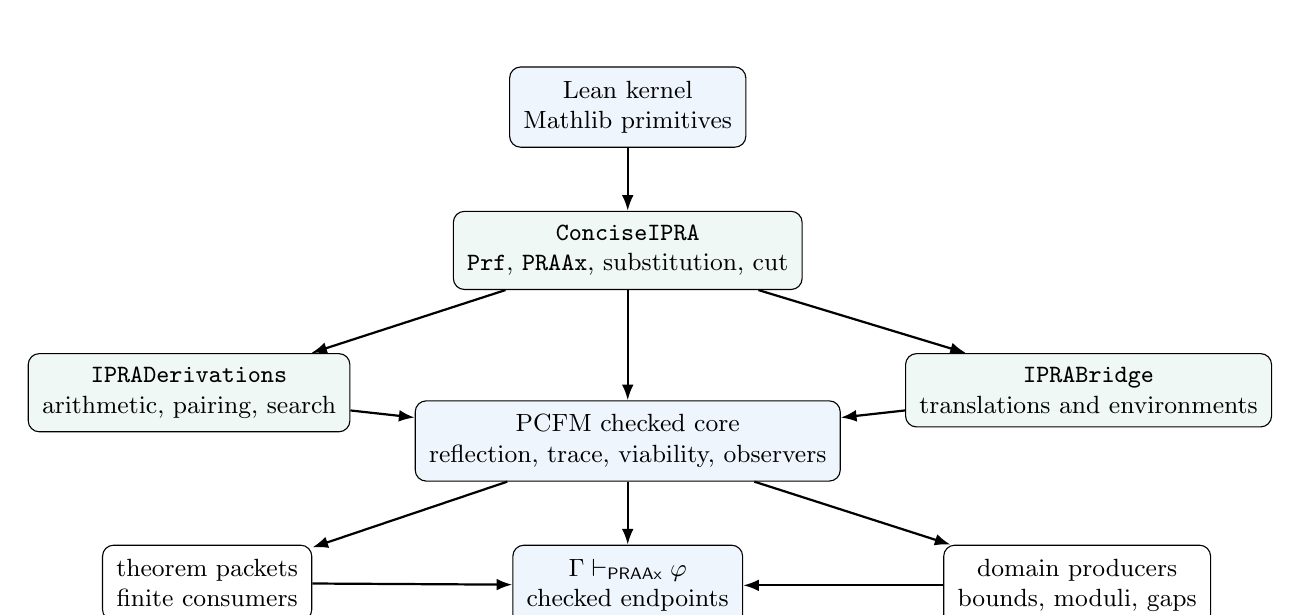
\begin{tikzpicture}[
  node distance=8mm and 13mm,
  box/.style={draw,rounded corners,align=center,inner sep=5pt,font=\small},
  arr/.style={-{Latex[length=2mm]},thick}
]
\node[box,fill=softblue] (kernel) {Lean kernel\\Mathlib primitives};
\node[box,fill=softgreen,below=of kernel] (concise) {\code{ConciseIPRA}\\\code{Prf}, \code{PRAAx}, substitution, cut};
\node[box,fill=softgreen,below left=of concise] (arith) {\code{IPRADerivations}\\arithmetic, pairing, search};
\node[box,fill=softgreen,below right=of concise] (bridge) {\code{IPRABridge}\\translations and environments};
\node[box,fill=softblue,below=14mm of concise] (pcfm) {PCFM checked core\\reflection, trace, viability, observers};
\node[box,below left=of pcfm] (packets) {theorem packets\\finite consumers};
\node[box,below right=of pcfm] (producers) {domain producers\\bounds, moduli, gaps};
\node[box,fill=softblue,below=of pcfm] (endpoints) {\(\Gamma\vdash_{\PRAAx}\varphi\)\\checked endpoints};

\draw[arr] (kernel) -- (concise);
\draw[arr] (concise) -- (arith);
\draw[arr] (concise) -- (bridge);
\draw[arr] (concise) -- (pcfm);
\draw[arr] (arith) -- (pcfm);
\draw[arr] (bridge) -- (pcfm);
\draw[arr] (pcfm) -- (packets);
\draw[arr] (pcfm) -- (producers);
\draw[arr] (packets) -- (endpoints);
\draw[arr] (producers) -- (endpoints);
\draw[arr] (pcfm) -- (endpoints);
\end{tikzpicture}
\end{center}

External Python tests and PDF prose are deliberately absent from the trusted
diagram.  They support development and review but do not justify an object
theorem.


\section{Proposed Lean signatures}
\label{app:signatures}

The notation below is schematic but tracks current repository names.  The
archive's \code{lean/} directory contains the same plan split into files.

\subsection{Structural modules}

\begin{lstlisting}[language={}]
namespace LeanProofs.IPRA.Framework

open LeanProofs.ConciseIPRA
open scoped Fm

structure Module (n : Nat) where
  req : List (Fm PTm n)
  out : Fm PTm n
  proof : req |- [PRAAx] out

namespace Module

def specialize (M : Module n) (sigma : Fin n -> PTm m) :
    Module m

def weaken (M : Module n) {Delta : List (Fm PTm n)}
    (h : List.Subset M.req Delta) :
    Delta |- [PRAAx] M.out

def discharge (M : Module n) {Delta : List (Fm PTm n)}
    (h : forall p, List.Mem p M.req -> Delta |- [PRAAx] p) :
    Delta |- [PRAAx] M.out

def closed {p : Fm PTm n}
    (h : ([] : List (Fm PTm n)) |- [PRAAx] p) :
    Module n
\end{lstlisting}

A unary contract may be a separate structure or an abbreviation:
\begin{lstlisting}[language={}]
structure Contract (n : Nat) where
  pre post : Fm PTm n
  sound : [pre] |- [PRAAx] post

def Contract.id (p : Fm PTm n) : Contract n
def Contract.comp (f : Contract n) (g : Contract n)
    (h : f.post = g.pre) : Contract n
\end{lstlisting}
An equality parameter in \code{comp} is avoidable by making pre/post explicit
arguments to the type.

\subsection{Boolean reflection}

\begin{lstlisting}[language={}]
def IsBool (b : PTm n) : Fm PTm n :=
  (b = 0) OR (b = 1)

def bnot (b : PTm n) : PTm n
def band (b c : PTm n) : PTm n
def bor  (b c : PTm n) : PTm n
def bimp (b c : PTm n) : PTm n

structure ReflectedQF {n : Nat} (phi : Fm PTm n) where
  bit : PTm n
  bool : ([] : List (Fm PTm n)) |- [PRAAx] IsBool bit
  true_iff :
    ([] : List (Fm PTm n)) |- [PRAAx]
      Fm.iff phi (bit = 1)
  false_iff :
    ([] : List (Fm PTm n)) |- [PRAAx]
      Fm.iff (phi --> Fm.bot) (bit = 0)

def reflectQF (phi : Fm PTm n) (hq : phi.QF) :
    ReflectedQF phi

theorem reflectQF_subst
    (R : ReflectedQF phi) (sigma : Fin n -> PTm m) :
    -- the reflected bit after substitution is provably equal
    -- to the substitution of R.bit
    ...
\end{lstlisting}

The compiler may return a dependent pair containing the QF proof rather than
accepting it separately.

\subsection{Bounded folds and search}

\begin{lstlisting}[language={}]
structure BoundedPredicate (k : Nat) where
  body : Fm PTm (k + 1)
  qf : body.QF
  reflected : ReflectedQF body

def allBit (P : BoundedPredicate k) : PR (k + 1)
def witnessF (P : BoundedPredicate k) : PR (k + 1)

theorem allBit_spec
    (P : BoundedPredicate k) :
    -- allBit N xs = 1 iff every i < N satisfies P
    ...

theorem witness_spec
    (P : BoundedPredicate k) :
    -- witnessF N xs < N iff a witness exists;
    -- returned witness satisfies P and is least
    ...
\end{lstlisting}

For an initial implementation, pack the \(k\) parameters into one natural code
and use the existing binary \code{Search.mu}.  A later generalized search can
avoid packing overhead.

\subsection{Traces}

\begin{lstlisting}[language={}]
structure TraceSpec (k : Nat) where
  run : PR (k + 1)
  runInv : Fm PTm (k + 1)
  runInvQF : runInv.QF
  zeroProof :
    ([] : List (Fm PTm k)) |- [PRAAx]
      runInv.subst (Syn.inst PTm.zero)
  succProof :
    [runInv] |- [PRAAx]
      runInv.subst
        (Syn.repl (PTm.succ (Syn.var 0)))

theorem TraceSpec.invariant (S : TraceSpec k) :
    ([] : List (Fm PTm (k + 1))) |- [PRAAx] S.runInv :=
  IPRA.ind S.runInv S.runInvQF S.zeroProof S.succProof
\end{lstlisting}

This low-level record exactly matches \code{IPRA.ind}.  A higher-level
constructor should generate \code{runInv}, \code{zeroProof}, and
\code{succProof} from a state transition and invariant.

\subsection{Stable observers}

\begin{lstlisting}[language={}]
structure BoundedWitness (n : Nat) where
  bound : PTm n
  good : Fm PTm (n + 1)
  goodQF : good.QF
  reflected : ReflectedQF good

structure ExactObserver (W : BoundedWitness n) where
  obs : PTm (n + 1)
  stable :
    -- two good witnesses below the bound have equal observations
    ...

theorem ExactObserver.select_spec
    (O : ExactObserver W)
    (nonempty : Gamma |- [PRAAx] boundedExists W.good W.bound) :
    -- least selected witness is good and its observation
    -- equals every good witness's observation
    ...
\end{lstlisting}

Setoid and metric observers replace equality in \code{stable}.

\subsection{Residual metadata}

\begin{lstlisting}[language={}]
inductive ObligationKind
  | local | resource | separation | certificate | external | bridge
  deriving Repr, DecidableEq

structure ObligationInfo where
  name : String
  kind : ObligationKind
  source : String
  note : String
  deriving Repr

structure PackagedModule (n : Nat) where
  module : Module n
  info : List ObligationInfo
  aligned : info.length = module.req.length
\end{lstlisting}

The alignment proof is bookkeeping only.  The formulas and \code{module.proof}
remain the trusted content.

\subsection{Bridge endpoints}

\begin{lstlisting}[language={}]
theorem codeNormalization
    (c : FoundationCode k) :
    referenceTheory |- forallClosure
      (apply c vars = apply (normCode c) vars)

theorem foundationFormulaRoundtrip
    (p : FoundationFormula ...) :
    referenceTheory |- p IFF
      toFoundation (toConcise p)

theorem standardToConciseCtx
    (h : Gamma |- [standardTheory] p) :
    mapToConcise Gamma |- [PRAAx] toConcise p

theorem conciseToStandardCtx
    (h : Gamma |- [PRAAx] p) :
    mapToStandard Gamma |- [standardTheory] toStandard p

theorem standard_concise_ctx_iff :
    (Gamma |- [standardTheory] p) <->
    (mapToConcise Gamma |- [PRAAx] toConcise p)
\end{lstlisting}

The exact Foundation notation should follow \code{IPRABridge}; these signatures
state the intended public surface, not replacement syntax.

\subsection{A compilation interface}

A shallow assembler need not define a universal graph.  A minimal interface is:

\begin{lstlisting}[language={}]
def use (M : Module n)
    (deps : forall p, List.Mem p M.req -> Delta |- [PRAAx] p) :
    Delta |- [PRAAx] M.out :=
  M.discharge deps
\end{lstlisting}

A later serialized graph can have:
\begin{lstlisting}[language={}]
structure WellTypedGraph (n : Nat) where
  goal : Fm PTm n
  residual : List (Fm PTm n)
  elaborate :
    residual |- [PRAAx] goal
\end{lstlisting}
In that form, the field \code{elaborate} already is the compilation theorem.
A parser or optimizer may construct the structure, but cannot inhabit it
without a proof.


\section{Audit checklist for future theorem packets}
\label{app:checklist}

Before a packet claims an iPRA theorem, answer every applicable question.

\subsection*{Endpoint}

\begin{enumerate}
\item What is the exact \code{Fm PTm n} conclusion?
\item What is the exact context of assumptions?
\item Is the endpoint a checked \code{Prf PRAAx}, a conditional checked
derivation, a host theorem, executable evidence, or a paper proof?
\item If a schema is intended, which parameters and precision queries index it?
\end{enumerate}

\subsection*{Representation}

\begin{enumerate}
\item What are the natural-number codes?
\item What is the validity predicate?
\item What equivalence relation represents mathematical equality?
\item Are all exported operations proved valid and extensional?
\item Is a claimed canonical representative actually computed and proved
canonical?
\end{enumerate}

\subsection*{Logic and induction}

\begin{enumerate}
\item Is every induction invariant quantifier free?
\item Have bounded quantifiers been compiled to finite folds or search?
\item Is any use of decidability restricted to reflected finite predicates?
\item Is a branch guard proved, rather than tested only in the host runtime?
\end{enumerate}

\subsection*{Resources}

\begin{enumerate}
\item What clock, search bound, modulus, height, gap, tail cutoff, cover radius,
or degree bound is used?
\item Is it a fixed PR term?
\item Where is its object-theory correctness proved?
\item If it is not proved, is it listed as a residual producer formula?
\item Has abstract finiteness been incorrectly treated as an effective bound?
\end{enumerate}

\subsection*{Witnesses and stability}

\begin{enumerate}
\item Is the output unique, setoid-unique, or only error-stable?
\item If a least finite witness is selected, is the selection compatible with
later refinement?
\item Does the theorem really need a coherent infinite selector?
\item Can a stable observable replace branch selection?
\item Is every exact sign, inverse, orientation, or root label guarded by a
separation certificate?
\end{enumerate}

\subsection*{Computation and certificates}

\begin{enumerate}
\item Is every computation a fixed primitive-recursive symbol or a bounded
clocked interpreter?
\item Are defining equations available in the object calculus?
\item If a trace is externally produced, is every transition checked inside
iPRA?
\item Does a host-level normalizer synthesize an object proof, or only prove a
Lean proposition?
\end{enumerate}

\subsection*{Composition}

\begin{enumerate}
\item Are local modules composed by \code{Prf.trans} or an equivalent checked
constructor?
\item Does substitution commute with the module's terms and formulas?
\item Are residual obligations aligned with their provenance ledger?
\item Can the final proof report its finite query support?
\end{enumerate}

\subsection*{Bridge and export}

\begin{enumerate}
\item Which backend contains the canonical theorem?
\item Is bridge transport needed only at the boundary?
\item Are free-variable environments documented?
\item Is the relevant term/formula round trip exact or only extensionally
proved?
\item Has a native or Foundation export been kernel checked after translation?
\end{enumerate}

\subsection*{Verification}

\begin{enumerate}
\item Does the Lean target build at the stated repository commit?
\item Are there any \code{sorry}, \code{admit}, new axioms, or opaque semantic
oracles?
\item Were Python tests labeled as evidence rather than proof?
\item Was the PDF rendered and visually inspected?
\item Does the README state limitations and remaining producer obligations?
\end{enumerate}

A packet that cannot answer one of these questions may still contain valuable
mathematics.  It should simply use the correct status label and expose the
missing boundary.


\begin{thebibliography}{99}

\bibitem{repo}
V.~Reshetnikov,
\emph{ProveIt: Logic/PrimitiveRecursiveArithmetic},
Git repository, baseline \texttt{7fa3ba48e8f62e8018ed954faaa48b908217eaf1},
16 November 2026.

\bibitem{concise}
V.~Reshetnikov,
\emph{Concise presentations of intuitionistic primitive recursive arithmetic},
ProveIt repository, \code{Logic/PrimitiveRecursiveArithmetic/ConciseIPRA}, 2026.

\bibitem{derivations}
V.~Reshetnikov,
\emph{iPRA derivations of theorems from the proof packets},
ProveIt repository, \code{Logic/PrimitiveRecursiveArithmetic/Derivations}, 2026.

\bibitem{bridge}
V.~Reshetnikov,
\emph{The Foundation--ConciseIPRA bridge},
ProveIt repository, \code{Logic/PrimitiveRecursiveArithmetic/Bridge}, 2026.

\bibitem{unification}
V.~Reshetnikov,
\emph{ProveIt iPRA unification plan},
ProveIt repository, \code{Logic/PrimitiveRecursiveArithmetic/UNIFICATION-PLAN.md}, 2026.

\bibitem{cbip}
V.~Reshetnikov and collaborators,
\emph{Certified Bounded Interaction Programs: A General Proof-Producing Framework for Mathematics in iPRA},
ProveIt research packet, 16 November 2026.

\bibitem{uniformity}
V.~Reshetnikov and collaborators,
\emph{Uniformity Gates and Bounded Refutation Frontiers},
ProveIt research packet, 15 November 2026.

\bibitem{bishop}
E.~Bishop and D.~Bridges,
\emph{Constructive Analysis},
Springer, 1985.

\bibitem{bridges}
D.~Bridges and F.~Richman,
\emph{Varieties of Constructive Mathematics},
Cambridge University Press, 1987.

\bibitem{troelstra}
A.~S.~Troelstra and D.~van Dalen,
\emph{Constructivism in Mathematics},
North-Holland, 1988.

\bibitem{kohlenbach}
U.~Kohlenbach,
\emph{Applied Proof Theory: Proof Interpretations and Their Use in Mathematics},
Springer, 2008.

\bibitem{kleene}
S.~C.~Kleene,
\emph{Introduction to Metamathematics},
North-Holland, 1952.

\end{thebibliography}
\end{document}
